\documentclass{deliverablereport}

\deliverable{hpc}{GAP-HPC-report}
\deliverydate{XX/YY/201Z}
\duedate{31/08/2019 (M48)}
\author{Author names}

\usepackage[backend=bibtex]{biblatex}
\addbibresource{report.bib}
\renewcommand{\comment}[1]{\TODO{Comment: #1}}
\begin{document}
\TODO{Author names}
\maketitle
% This will be the abstract, fetched from the github description
\githubissuedescription

\newpage
\tableofcontents

% write the report here

% Original list of sections and subsections created from
% https://github.com/OpenDreamKit/OpenDreamKit/issues/113

\TODO{The material we actually expect them to read -- ie not tables
  and appendices should probably not exceed 15 pages, so we may need
  to be a bit more selective, or find ways to say things more
  concisely. At the very least we need to steer them clearly to the
  important messages, with the detail there for them to dig into if
  they want to.}

\TODO{Have we got better macros for including code than simple LaTeX
  verbatim? AK: tried some but so far did not like the font there}

\TODO{If time permits -- I'll try and talk to some of the others
  tomorrow, but we can also look at the other reports -- it would be
  nice to link some of our experiences/decisions/activities to similar
  developments in other systems (or even contrast them to different
  ones), pushing tyhe message of coming togethert in \ODK}

\section{Introduction}
\TODO{get HPC in earlier and mention that other deliverables that \GAP
  is involved in are extremely focused, which is another reason why
  this one includes the broad stuff}
This report describes the work undertaken in connection with Task~5.2,
which covers developments within the \GAP system to meet the general
objective of workpackage 5 (High Performance Mathematical
Computing), to ``improve the performance of the computational
components of OpenDreamKit'' on  a wide range of architectures,
relevant to current and prospective users. We have worked on
supporting use of a range of High Performance Computing environments,
prioritising those most accessible to our users, namely multicore
systems, clusters and cloud computing. We have also made
fundamental performance improvements that benefit all \GAP users.

In a system such as \GAP, which is actively developed by a widely
distributed team, only a few of whom are part of the \ODK project, any
developments which are to be useful to users of \GAP (whether as a component of
\ODK or not) need to be maintainable, and
integrate well with the general flow of \GAP development, which itself
has to be nurtured and supported. Because of this, it is neither
possible nor desirable to clearly delineate every development which
is part of Task~5.2 from every one which is not. On the other hand,
the impetus and resources from the \ODK project have meant that \ODK
goals have pervaded a great deal of \GAP's evolution over the last
four years.

In the light of this, this report will necessarily take the form of  a broad
survey of all the major developments in \GAP and its package ecosystem
over the period, but we will concentrate on, and highlight, links between
these developments and \ODK goals. Work which is specifically part of
other work packages is reported in appropriate deliverables, but these
are mainly quite focused, leaving a broad range of material for this report.

\subsection{Context and Background}

Recall that \GAP (``Groups, Algorithms, Programming'') is a software system for
computational discrete mathematics, with its origins in finite group
theory. The system has been developed continually since 1986, with the
first public release in 1988. Throughout its life it has been made
available free of charge for use, extension and non-commercial
redistribution. It is widely used by researchers in mathematics,
computer science and other disciplines, and has been cited in
\href{https://www.gap-system.org/Doc/Bib/bib.html}{almost 3000
  research papers}. It is also widely used in teaching.

Thus far, \GAP has
normally been used via a single-threaded text-based ``read-eval-print-loop'' UI, with the
same \GAP language serving both for the interface and for the
implementation of much of the system. A research user 
may use the system purely interactively, as a ``desk calculator'', but
typically will extend the system with a small or large collection of
\GAP functions and complete their research calculations by interacting
with those. One of the goals of \GAP related work in \ODK is to offer
a range of flexible alternatives to this in line with current
practices in other areas, and more suited for modern high-performance
computers.

A key feature of \GAP today is the rapdily growing ecosystem of
contributed extensions called ``packages'' (145 are redistrubuted with
\GAP 4.10.2). These packages may: extend mathematical functionality of
the system by implementing new algorithms; provide mathematical
datasets, together with search and access functions or provide
enhanced tools for users and/or developers. Packages can be published
independently of the core \GAP system and each has a separate
authorship. For the last decade or more, the majority of the
development work in the \GAP ecosystem has been in packages.
Another area of \GAP development under \ODK is to ensure
that the package system (including the infrastructure used to gather,
test and release packages) scales as the number of packages grows.


Prior to the start of \ODK, a number of initiatives had developed
alternative models for the use of \GAP. \SageMath (\Sage hereafter)
has used \GAP for much of its group theoretic functionality since
2006. One benefit of that was that it allowed the use of \GAP
functionality through \Sage's notebook UI.In the Framework~6 project
``SCIEnce: Symbolic Computation Infrastructure for Europe'' we
developed a poweful and flexible remote procedure call interface to
\GAP using the \href{??}{OpenMath} data representation format, called
SCSCP (Symbolic Computation Software Composability Protocol) one of
whose roles was to support coarse-grained distributed computation. In
a UK-funded software development project: \HPCGAP, we began the
development of an intrinsically multi-threaded version of \GAP. As
well as new software, these projects gave us insight into the parallel
and high-performance computing needs of our user community, leading
us, for instance, to remain more focused on multicore servers and
\textit{ad hoc} clusters (such as a mathematical research group or
department might provide) than on ``supercomputers''. Even on these
systems, interactive use rather than ``batch'' computation remains the
norm, and we aim to support that, and enhance it through Jupyter
notebooks rather than force users to a model that does not suit them.

The central thrust of the involvement of \GAP in \ODK is increased
diversity of users and models of use. To this end, in WP3~we have
added support for direct use of \GAP via Jupyter notebooks as an
alternative to our 1980s text-based UI. In this work package we report
work intended to support \GAP users in performing larger and more
demanding computations. This includes general work on increasing the
performance and robustness of \GAP and its packages, continued
development of our support for shared memory parallel computing via
\HPCGAP and MeatAxe64 and for distributed memory parallel computing
via SCSCP. We also report enhancements to the \GAP language and to
\GAP's development and debugging tools and our upport for package
developers. More demanding computations requires more complex software
to be written, debugged, optimised and shared, and these changes
enable that.

\subsection{Overview}
\TODO{Put the sections in a logical order with the best stuff and most
  WP5 relevant stuff at the
  front. Adjust this para accordingly}
This report is divided into sections as follows: the next section (\ref{core-gap})
reports relevant general developments in the core \GAP system. Section
\ref{hpc-gap} focuses on developments in the multi-threaded
system. Section \ref{gap-infra} discusses our work aimed at improving
robustness and reliability, both of \GAP and its packages. This
includes both new tool support and new processes. Section
\ref{packages} reports on new and enhanced packages relevant to the
objectives of this work package.  Section \ref{sec:jupyter} reports
additional developments in the use of Jupyter as a \GAP interface,
since the last relevant deliverable of WP3.

\TODO{Finish this when the later sections stabilize}


\section{Developments in the core \GAP system}\label{core-gap}

This Section highlights some of the most important
changes to the core \GAP system released
during the project which contribute to \ODK goals. Other important developments are
included in \GAP packages and described in later sections.  More
detailed descriptions of each major and minor \GAP release, with links
to the corresponding source code changes on GitHub, are contained in
the ``GAP - Changes from Earlier Versions'' document. This document is
redistributed with \GAP and is also available on the \GAP website at
\url{https://www.gap-system.org/Manuals/doc/changes/chap0.html} and
included as an appendix to this3 report.

This work includes many contributions from collaborators outside \ODK,
whose authorship can be seen from the version control history.
\TODO{Remember to add Changes (and HPC-GAP) manuals as an appendix}

\comment{I wonder if we should use ODK month numbers as well as, or
  instead of, actual dates. Similarly USTAN instead of ``St Andrews''?
  AK: for the Commission, yes; for the reader that will be less clear
  and then perhaps should be explained in the preamble. SL I suggest
  explaining them in a footnote the first time we use them -- that
  USTAN is St Andrews, and when month 0 was.}

\subsection{\GAP 4.8 (February 2016)}\label{gap-4.8}

\TODO{We should be consistent in terminology -- do we release versions
  or publish releases? AK: I would then prefer ``publish release'' (so that
  ``latest public release'' and ``major release'' 
  sounds nicer than ``latest public version'' and ``major version''.
  But we still can use ``release'' as a verb, e.g. ``we released GAP 4.10.2''.}

\GAP 4.8 was the first major release of \GAP published
after the start of the \ODK project. 
As a preparation for the planned integration of \HPCGAP branch
(supporting \GAP language level threading) into
the core system some language extensions were backported to core
\GAP at this stage. 
\TODO{very briefly say what they were.
AK: mainly \url{https://github.com/gap-system/gap/tree/master/lib/hpc}, see this:}
This helped to unify the codebase of both \GAP~4 and \HPCGAP
by allowing to read \HPCGAP code in a single-threaded
\GAP session. The only not backwards compatible change is that 
\verb|atomic|, \verb|readonly| and \verb|readwrite| became keywords
and are no longer valid identifiers.

In addition, this release also provided support for much enhanced
profiling, essential to all our performance engineering work.
Previously \GAP\ allowed tracking of the CPU time spent
executing each function, but the new features in this release
reduced this granularity to individual lines of \GAP
code. Related developments also made it easier to track time spent on
individual lines of C code in the \GAP kernel. A further related
feature makes it very easy to measure ``test coverage'' -- the
proportion of the system that has actually been executed by a given
set of tests. The {\sf Profiling} package \cite{profiling} by Christopher Jefferson (St
Andrews) provided excellent tools for transforming these profiles into
various human-readable forms. These features supported later work on
enhancing both the performance and the reliability of \GAP, through
easier identification of hot-spots and easier measurement of test
quality.

This release also included some language extensions which would allow
users to write more efficient and readable code:

\begin{itemize}
  \item support for \emph{partially
  variadic functions} similar to those allowed in Python, allowing
function expressions like
\verb|function( a, b, c, x... ) ... end;|
which requires at least three arguments \verb|a|, \verb|b| and
\verb|c| and assigns the first three to \verb|a|, \verb|b| and \verb|c|
and then a list containing any remaining ones to \verb|x|.
\item more flexible list indexing, allowing users to install methods
  for multiple indexing (\verb|m[i,j]| instead of \verb|m[i][j]| for
  arrays) and more varied indices (such as \verb|l[-1]| to access a
  doubly-infinite virtual list \verb|l|). As well as being more
  flexible, this is a step towards supporting more efficient array
  implementations in which ``row objects'' (like \verb|m[i]| in
  \verb|m[i][j]|) might not exist.
\end{itemize}

\GAP 4.8 had seven public releases between February 2016 and August 2017, and
was replaced by \GAP 4.9.

\subsection{\GAP 4.9 (May 2018)}\label{gap-4.9}

\GAP 4.9 continued the restructuring and modernising of the core \GAP
system, aiming at the greater reliability, flexibility and performance
which would be needed for \GAP users to gain the full advantage of the \ODK ecosystem.
For example, we removed our old home-grown large integer arithmetic
implementation, and committed fully to the state of the art external
library \href{???}{GMP}. This
move continues our cautious programme of exploiting existing free
software in our core system. Our caution here is based on
experience. Moving too quickly in this area in the past has created
problems with the reliability and
portability of \GAP on which our users depend.

This release incorporated a completely
reimplemented build system for \GAP, using more modern tools and
complying with modern expectations. This resolved many issues with the
old system, and made it easier to maintain and extend. For example it
makes it much easier to maintain multiple configurations of \GAP on a
single system from a single copy of the source. Technical
details of the new build system are described in {\tt
  README.buildsys.md} from the \GAP source code. Crucially the new build system
was the final prerequisite for the planned  merge of the \HPCGAP codebase  into the
mainstream \GAP system as a compile-time option (for details, see
Subsection~\ref{hpc-gap}).

An additional benefit of the new build system is that it makes it much
easier to robustly include C or C++ extensions to the \GAP kernel in
contributed packages, including interfaces to many free C and C++
libraries. By making it easy to accelerate bottleneck steps, this
greatly enhanced the overall performance of many packahges, while a
encouraging integration of existing libraries in packages complements
our cautious approach mentioned above to including them in the core
system. \TODO{SL: I more or less just made this up, but I think it's
  true. Can we find any examples? AK: semigroups, with libsemigroups
  as a library, is a good example, in which James collaborated with
  ODK partners in France; another example may be curlInterface, which 
  then became very useful to Michael's PackageManager.}

This release also incorporated many smaller performance improvements. For example,
\GAP now supports named constants, whose value cannot change 
at runtime. While maintaining readability through naming, uses of
these constants can be optimised as a function is parsed, so that they
are at least as fast as using explicit values. Another notable improvement was
to the widely used  sorting functions which now use the best
recently published algorithms and were also made more maintainable by
restructuring the implementation.

Debugging  and profiling tools were also improved based on experience with
\GAP 4.8. Further changes improved \GAP
usability by allowing more efficient and/or readable code, in line
with other modern programming languages:
\begin{itemize}
  \item a concise syntax for short
    functions with any number of arguments, so that, for example,
    \verb|{a,b} -> a+b| abbreviates \verb|function(a,b) return a+b; end|. 
\item more flexibility in \GAP expression syntax,
  where previously there were annoying technical restrictions. For
  example, an entry of the sum of two vectors can now be accessed as
  \verb|x := (v+w)[i]| instead of \verb|u := v+w; x := u[i]|.
  
%%   use of function literals in expressions such \verb|y := f().x;|
%% replacing previously required two-step calculation
%% \verb|y := f();; y := y.x;|.
%% This -- and the release
%%   announcement -- are actually wrong! This syntax always worked, the
%%   example in the PR is \verb|(f()).x| which is different}

\end{itemize}

\GAP 4.9 had three public releases between May and September 2019, and
was replaced by \GAP 4.10.

\subsection{\GAP 4.10 (November 2018)}\label{gap-4.10}

The release of \GAP 4.9 with the new build system allowed the
restructuring of the core \GAP system to continue, and allowed us to
finalise a number of other ongoing changes, leading to \GAP 4.10
after a shorter than usual interval. \GAP 4.10 is current
version of \GAP, with the latest release being \GAP 4.10.2, published
in June 2019 and \GAP 4.11 expected in November 2019.

The most important new feature in \GAP 4.10 was the first pubolci
release of \texttt{libGAP}: an
option to compile \GAP as a C library instead of a stand-alone
executable. This is very important for many uses of \GAP in \ODK and
is discussed further in section \ref{libgap} below.

\GAP 4.10 also provides experimental support for using alternative
memory management systems, notably the \href{??}{Julia} garbage
collector and the \href{???}{Boehm garbage collector}, in place of the
GASMAN system which was developed for \GAP 4 in the 1990s.  These
garbage collectors are thread-safe (important for \HPCGAP) and the
option to use the Julia garbage collector will allow tight integration
of \GAP with Julia programs and other systems via Julia. Use of Julia
in this way is an initiative led by the
\href{https://oscar.computeralgebra.de/}{OSCAR} project, developed
within the DFG-funded grant SFB-TRR 195 ``Symbolic Tools in
Mathematics and their Application'' and is seen as complentary to \ODK.

The work on improving debugging and profiling in \GAP has
continued. Profiling now reports memory usage as well as CPU time, and
additional checking options (both internal and by using external tools such as
\href{???}{valgrind}) help to detect misuse of memory in the kernel.

Using the improved debugging and profiling facilities we were able to
detect many performance bottlenecks and confirm that new code
genuinely improved performance, as well as detecting many bugs much
earlier in the development process. To alleviate performance
bottlenecks in key applications, we rewrote much of the method
selection (dispatch) code \GAP to C and gained large speedups by
reengineering many integer arithmetic functions.

\TODO{fix long line below}

For example, the table below gives the CPU time in milliseconds required
to run \verb|for i in [1..k] do x:= 1/p^q mod n; od|

\begin{center}
\begin{tabular}{| c | c | c | c | c | c |} 
\hline
p & q    & n          & k        & ms, before & ms, after \\
3 & 60   & $2^{59}$   & 2000000  & 2364       & 1219 \\
3 & 60   & $2^{60}$   & 2000000  & 2821       & 1292 \\
2 & 6000 & $3^{6000}$ & 6000     & 19358      & 692  \\
\hline
\end{tabular}
\end{center}

%Before
%gap> q:=1/3^60;;n:=2^59;; for i in [1..2000000] do x:= q mod n; od; time;
%2364
%gap> q:=1/3^60;;n:=2^60;; for i in [1..2000000] do x:= q mod n; od; time;
%2821
%gap> q:=1/2^6000;;n:=3^6000;; for i in [1..6000] do x:= (q mod n); od; time;
%19358
%
%After:
%
%gap> q:=1/3^60;;n:=2^59;; for i in [1..2000000] do x:= q mod n; od; time;
%1219
%gap> q:=1/3^60;;n:=2^60;; for i in [1..2000000] do x:= q mod n; od; time;
%1292
%gap> q:=1/2^6000;;n:=3^6000;; for i in [1..6000] do x:= (q mod n); od; time;
%692

\TODO{Maybe drop this next one, a bit technical? AK: maybe (mention only last
line maybe - enables calculation not easily doable in default memory settings before?}

Also, \verb|InverseMatMod| with integer modulus has been improved.% #2426
The following table shows the runtime needed to call
\verb|x:=InverseMatMod(m,q);| a hundred times for a random unimodular $100 \times 100$
matrix \verb|m|:

\begin{center}
\begin{tabular}{| c | c | c |} 
\hline
q     & ms, before    & ms, after \\
\hline
2     & 277           & 273 \\
251   & 1564          & 1249 \\
65537 & out of memory & 1226 \\
\hline
\end{tabular}
\end{center}

%Before:
%
%gap> m2:=RandomUnimodularMat(100);;
%gap> for i in [1..100] do x:=InverseMatMod(m2,2); od; time;
%277
%gap> for i in [1..100] do x:=InverseMatMod(m2,251); od; time;
%1564
%gap> for i in [1..100] do x:=InverseMatMod(m2,65537); od; time;
%Error, reached the pre-set memory limit
%
%After:
%
%gap> m2:=RandomUnimodularMat(100);;
%gap> for i in [1..100] do x:=InverseMatMod(m2,2); od; time;
%273
%gap> for i in [1..100] do x:=InverseMatMod(m2,251); od; time;
%1249
%gap> for i in [1..100] do x:=InverseMatMod(m2,65537); od; time;
%1226

The same improved profiling tools identified other
``hidden'' bottlenecks in \GAP code. For instance \GAP has a
sophisticated system of inference that can trigger 
so-called ``immediate methods'': quick attempts to deduce additional
consequnces from information that becomes known about an object.
In general, these are very effective, and the deduced information can
lead the system to chose better methods for subsequent
calculations. For instance, when a group learns its order, if that
order is finite and odd, then by the celebrated
Feit-Thomson theorem the group must be solvable. Once that
is known, much more efficient methods can be applied for many
subsequent calculations.

While this is a very powerful feature in most situations, in some
calculations, a large number of short-lived objects are created,
and the immediate methods use a great deal of time deducing knowledge
about each of them
that will never be used. The profiling developments made this 
easily visible for the first time, and some small adjustments to the
immediate methods produced up to a six-fold speed up in fundamental
operations such as computing isomorphism groups. For instance, the
run-time for the code fragment below dropped from 130
seconds to 22.


{\Small
\begin{verbatim}
G:=PcGroupCode( 
  741231213963541373679312045151639276850536621925972119311,
  11664);;
IsomorphismGroups(G,PcGroupCode(CodePcGroup(G),Size(G)))<>fail;
\end{verbatim}
}

\TODO{Can we claim that the smaller number of minor releases (and the
  dropping of the .0 beta for each major release) are due to the
  better testing tools? If so, is this the place, or can we refer
  forward where we talk about those tools above? 
  AK: we can say something - perhaps not about the smaller number
  (if compare 2012-2015 vs 2016-2019, it's in the same range), 
  but of less changes in minor releases, and of dropping the beta too; 
  I think better to refer forward, see the section about distributions}

\subsection{\GAP 4.11 (anticipated in November 2019)}\label{gap-4.11}

% Since they are released on GitHub, I see no reason not to also
% highlight changes which are merged and definitely coming out in
% 4.11, if they are relevant SL

% Release notes are collected at https://github.com/gap-system/gap/wiki/GAP-4.11-release-notes

At the time of preparation of this report, the next major release,  \GAP
4.11, is approaching completion. Almost all of the features to be
included in it (including all the ones highlighted here) are already
publicly  available on GitHub to developers or anyone else interested.

One important and relevant feature of this release will be the ``syntaxtree'' reflection
API for \GAP, allowing \GAP programs to access and modify the internals of \GAP
functions, opening up a range of possibilities for optimisation, automatic
parallelisation, and more effective compilation into C. This is
discussed in more detail in section \ref{syntaxtree} below. 

Additional relevant features are continued improvements to debugging and
profiling facilities (for example,
%#2772 
adding support for profiling interpreted code
and 
%#3420
making profiling reports more informative by 
giving more library methods human-readable names;
%#2900 
allowing to abort \verb|Test| by pressing ctrl-C;
%#1633 
allowing local variables in test files via
\verb|#@local <list of variables>|,
and conditional execution of tests via \verb|#@if|, \verb|#@else|, \verb|#@endif|.

The \texttt{libGAP} API has been extended
to allow programs using the system in this way
more convenient access to \GAP objects such as
%#2998, #2999, #3007 
characters, floats, integers
%#3554
and matrices; 
%#3516
the performance of Julia GC integration also improved,
%#3335 
and the memory usage on Windows when running external programs was reduced.

Further performance enhancements included, among others,
%#3579 
speeding up writing to global variables;
%#3566 
optimising operations involving identity permutations;
%#3231 
speeding up \verb|IsConjugate| for \verb|IsNaturalSymmetricGroup|,
%#2924 
improving performance of \verb|NormalizerViaRadical|,
%#3031 
and of \verb|ConjugacyClasses| for solvable groups. For example, the time
of the following calculation reduces from 110 seconds to 53 seconds:

{\Small
\begin{verbatim}
G:=WreathProduct(CyclicGroup(IsPermGroup,12),DihedralGroup(IsPermGroup,12));
ConjugacyGlasses(G);
\end{verbatim}
}
\noindent


\comment{%#3370 
Pragmas are now available
(this is useful for syntaxtrees)
}

% What about making pages for relevant releases in
% https://www.gap-system.org/Manuals/doc/changes/manual.pdf 
% (or print HTML version of the manual into PDF)
% an electronic appendix to the deliverable?
%
% Yes -- let's do that. Add them as appendices.
%
% Indeed, as the ODK README.md says:
%
%  The report shall be self-contained. Indeed, the
%  deliverable will be evaluated based upon its version submitted on
%  the EU portal without retrieving other resources. Links have no
%  legal value, since there is no guarantee that the referenced
%  material will remain unchanged. One may typically want to add
%  relevant material as appendix (e.g. snapshots of software
%  documentation, websites, or other relevant documents); see e.g.
%  [WP5/D5.1/report.tex](WP5/D5.1/report.tex) or
%  [WP2/D2.1/report.tex](WP2/D2.1/report.tex).

\TODO{Can we assemble some statistics to show the general progress of
  work on \GAP performance and robustness over the project -- number
  of tests, maybe run the 4.8 or 4.7 testinstall in 4.7 and 4.11 and
  compare performance?}

%% \comment{tests from 4.7.9 take 3237s in GAP 4.7.9;
%% 4.10.2: total 3039s (150s GC) and 328GB allocated;
%% GAP master: total 2913s (140s GC) and 293GB allocated}

As one example of the general effectiveness of our performance
improvements, the full test suite of \GAP 4.7.9 (current at the
start of the project) which takes 3237 seconds to run on \GAP 4.7.9 on
current hardware, runs unchanged in just over 2900 seconds with a
pre-release version of \GAP 4.11. Many of the most widely used and
important areas of \GAP functionality have seen bigger changes.  

% find . -name '*.tst' | wc -l
% find . -name '*.tst' | xargs wc -l

As an example of the increased robustness of the system, the table
below shows the development of our test suite over this period.

\begin{center}
\begin{tabular}{| l | l | c | c |} 
\hline
GAP release & Release date & Number of test files & Number of lines \\
\hline GAP 4.7.8  & November 2015           & 69 & 21981 \\
\hline GAP 4.8.10 & January 2018            & 91 & 28586 \\
\hline GAP 4.9.3  & September 2018          & 564 & 41456 \\
\hline GAP 4.10.2 & June 2019               & 648 & 53362 \\
\hline GAP 4.11   & expected November 2019  & 707 & 61280 \\
\hline
\end{tabular}
\end{center}

\subsection{libGAP: allowing 3rd party code to link \GAP as a library}\label{libgap}

The initial connection between \Sage and \GAP was developed around
2006, and relied on running a full \GAP process with which \Sage
communicated through UNIX pipes, creating \GAP input as text and then parsing
the text which was output from \GAP. This enabled an initial connection, but
introduced considerable overhead converting objects to and from text
representations and passing them between processes, and considerable
unreliability, since \Sage was essentially using \GAP through an
interface designed for humans, rather than programs.

A better solution is to provide a C API enabling \GAP to be integrated
into the \Sage process, and allowing a \GAP session to be started,
objects created, functions called and results retrieved via C function
calls. This is, however, not a mode of operation for which \GAP was
ever designed, and implementing it in a robust and flexible way
required considerable adaptations to the system, essentially
disentangling the computational engine from the UI, while retaining,
for example, the ability to dynamically load C code from \GAP
packahges into the process that was using libGAP. Another complication
is the need to make sure that the \GAP memory manager does not delete
objects which the calling process will want in the future.

Based on an iniital version developed within the \Sage team, a fully
general-purpose and flexible version was released in \GAP 4.10.0
(November 2018).

Subsequent releases have improved and will continue to improve the
robustness of libGAP, and to extend its API with new functionality (See Chapter 2 
``Changes between \GAP 4.9 and \GAP 4.10'' of the 
``\GAP - Changes from Earlier Versions'' manual for the detailed
descriptions). This has allowed \Sage to drop its custom 
modifications to \GAP and use an official, documented and regularly 
tested \GAP interface instead, starting from SageMath 8.6 (January
2019).

% See SageTrac ticket 22626 made that happen; it was merged in 
% SageMath 8.6.beta0, so SageMath 8.6 had it but not SageMath 8.5.

\subsection{Reflection}\label{syntaxtree}
\TODO{SL: write this}

\section{High-performance computing with \GAP}\label{hpc}

\subsection{\HPCGAP: multithreaded programming in \GAP}\label{hpc-gap}

\GAP 4.9.1 (May 2018) for the first time included experimental code to 
support safe multithreaded programming in \GAP, dubbed \HPCGAP. This
had been in development for some time as a fork of \GAP and the \HPCGAP and \GAP
codebases had diverged. In this release we reunified them,
making thread support a compile-time option instead of requiring a completely
different programme. This was an essential step to support further development of 
\HPCGAP, and ensure that new developments in \GAP could be quickly
incorporated. It also provided general \GAP users an opportunity to start to experiment 
with \HPCGAP, for which documentation is also provided.

\HPCGAP supports two models of parallel programming in \GAP, which can
be combined: threads and tasks. Threads operate as in most languages.
The basic primitive is to start execution of a \GAP function in a new
thread, while the calling thread returns immediately. Threads can
interact through global data or by returning results when they exit. A
range of mechanisms and data structures are provided for threads to
interact safely. Tasks are
similar, but they are submitted to a shared job queue and executed by
one of a fixed-size pool of worker threads. Typically the calling
process will start a number of tasks and then wait for some or all
of them to complete.  Supporting these models efficiently required considerable work on
the \GAP interpreter, but was otherwise straightforward.

One of the main challenges in \HPCGAP, however, is that the \GAP
library makes very extensive use of shared global data, which is
frequently updated as new knowledge is obtained. Removing this sharing
of knowledge would make the overall system much less effective, as
well as requiring millions of lines of code to be rewritten, but
ensuring that access and updates to this data from different threads
and tasks did not cause corruption or inconsistency was difficult.

The approach taken was to limit access, in most cases, to
data ``owned'' by the accessing thread, read-only data and ``public''
data stored in thread-safe data structures which were used for the
global ``knowledge pool''. This is implemented by
access checks in the kernel with the aim of ensuring that most unsafe
data access should result in error messages, rather than inconsistent
results. Experiments with this system have been reported in a number
of papers for instance \cite{something}.
\TODO{e.g. something from \url{https://scholar.google.co.uk/scholar?oi=bibs&hl=en&cites=17020645280914341716&as_sdt=5}}

The main remaining challenge is to adapt the enormous legacy codebase
represented by \GAP's library and key packages to use these mechanisms
effectively, and to keep the underlying mechanisms working as the core
\GAP codebase evolves. Fusing the codebases, as was done in \GAP 4.10
was a critical step in this work, meaning, for instance, that all
changes to \GAP are tested in \HPCGAP automatically.

The effectiveness of the underlying task mechanism is illustrated in
the graph below, which shows the speedups (wall-clock time on $n$
cores versus CPU time on one core) achieved in running 1000 test tasks
(each taking about 300ms) with various numbers of worker threads on a 64
core AMD ``bulldozer'' system. These cores share L2 cache and decode
hardware in pairs, limiting performance with larger numbers of
threads.

\begin{figure}[!ht]
    \centering
    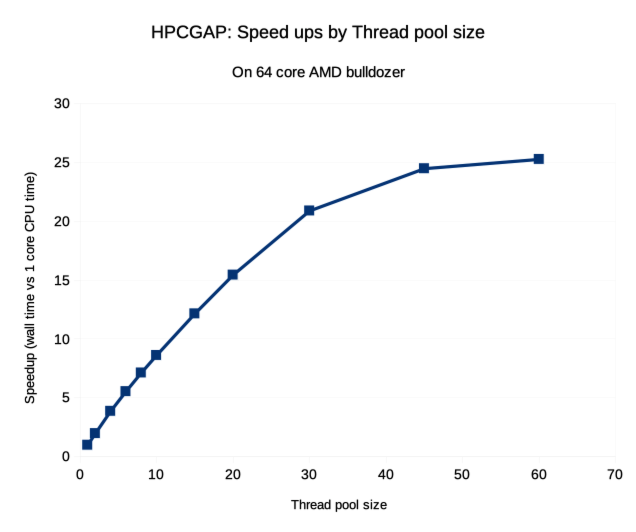
\includegraphics[width=0.8\textwidth]{images/hpcgap-speedups}
    \label{fig:hpcgap-speedups}
\end{figure}


% Release announcement: https://www.gap-system.org/Manuals/doc/changes/chap3.html#X7F52B77B7DBACC17

% \HPCGAP manual: https://www.gap-system.org/Manuals/doc/hpc/chap0.html

% What about making https://www.gap-system.org/Manuals/doc/hpc/manual.pdf 
% an electronic appendix to the deliverable?

\subsection{meataxe64: high-performance linear algebra over finite fields}\label{meataxe64}

A key kernel for many applications of \GAP is linear algebra for
mainly dense matrices over
a range of finite fields, especially small ones. This is used directly in working with
matrix groups and in computational representation theory, but also
arises indirectly in areas such as graph theory, finite solvable
groups and number theory. \TODO{maybe explain a bit how lionear
  algebra over small finite fields is different from floating point or
  exact} The \GAP kernel includes memory-efficient
representations of matrices over these fields, and implementations
based on the C-meataxe (the name ``meataxe'' is derived from the
abbreviation ``mtx'' for ``matrix'' and the fact that a key operation
in computational representation theory is to ``chop'' a module into
its irreducible components).

Working with external collaborators (primarily R.A.~Parker),
we have supported (and continue to contributeto ) the design and development 
of a new C and
assembler library, called ``meataxe64'' which takes
advantage of new algorithmic ideas, and of powerful features of modern
CPUs, to deliver a quantum leap in performance. We have implemented a
\GAP interface to it (the ``meataxe64 \GAP package'' \cite{meataxe64}) currently in
beta-test, and are in the process of revising higher levels of the software stack to make best
use of it.

The meataxe64 C library is multi-threaded and can make very efficient
use of multiple cores for large enough matrices, whether used from
\HPCGAP or regular \GAP.

Tables \ref{fig:matmult:gap}, \ref{fig:matmult:mtx64},
\ref{fig:matmult:par} indicate the performance gains and
speedups obtained by meataxe64 compared to our existing code.  The
data is based on run-times for multiplication two random dense
square matrices of the given dimension with entries from $GF(q)$. In
these tables the throughput is calculated as the cube of the dimension
divided by the elapsed (``wall-clock'') time, ignoring algorithmic
techniques that may reduce the action number of field operations
needed. The unit (Gfop/s) is billions of field operations per second.

\begin{small}
\begin{center}  
  \begin{longtable}{|c|c|c|c|c|}
\caption[]{Performance of existing \GAP code}\label{fig:matmult:gap}\\
    \hline
    $q$&Dim.&cpu (s)&wall (s) &throughput (Gfop/s)\\
    \hline
    \endhead
    \hline
    \endfoot
2&800&0.004&0.003&149.6\\
2&1600&0.016&0.016&255.8\\
2&4000&0.159&0.159&401.7\\
2&8000&1.581&1.582&323.6\\
2&16000&14.241&14.280&286.8\\
2&40000&193.251&193.524&330.7\\
3&500&0.053&0.052&2.4\\
3&1000&0.364&0.364&2.8\\
3&2500&5.268&5.268&3.0\\
3&5000&41.529&41.533&3.0\\
3&10000&327.798&328.121&3.0\\
3&25000&5020.887&5025.466&3.1\\
4&400&0.017&0.017&3.8\\
4&800&0.112&0.112&4.6\\
4&2000&1.542&1.542&5.2\\
4&4000&12.107&12.108&5.3\\
4&8000&99.259&99.361&5.2\\
4&20000&1513.64&1515.528&5.3\\
5&300&0.021&0.021&1.3\\
5&600&0.147&0.148&1.5\\
5&1500&2.166&2.166&1.6\\
5&3000&17.106&17.108&1.6\\
5&6000&136.714&136.840&1.6\\
5&15000&2088.063&2089.934&1.6\\
7&200&0.009&0.009&0.9\\
7&400&0.063&0.062&1.0\\
7&1000&0.906&0.906&1.1\\
7&2000&7.32&7.321&1.1\\
7&4000&56.659&56.710&1.1\\
7&10000&875.08&875.901&1.1\\
16&200&0.007&0.007&1.2\\
16&400&0.044&0.044&1.4\\
16&1000&0.644&0.643&1.6\\
16&2000&4.978&4.978&1.6\\
16&4000&39.757&39.798&1.6\\
16&10000&628.858&629.651&1.6\\
17&100&0.003&0.003&0.4\\
17&200&0.018&0.018&0.4\\
17&500&0.273&0.273&0.5\\
17&1000&2.153&2.154&0.5\\
17&2000&17.119&17.131&0.5\\
17&5000&268.032&268.267&0.5\\
64&100&0.002&0.002&0.5\\
64&200&0.012&0.013&0.6\\
64&500&0.186&0.186&0.7\\
64&1000&1.448&1.448&0.7\\
64&2000&11.548&11.558&0.7\\
64&5000&294.897&297.453&0.4\\
81&100&0.003&0.003&0.4\\
81&200&0.019&0.019&0.4\\
81&500&0.284&0.284&0.4\\
81&1000&2.215&2.215&0.5\\
81&2000&21.285&21.353&0.4\\
81&5000&276.045&276.503&0.5\\
101&100&0.003&0.003&0.3\\
101&200&0.021&0.020&0.4\\
101&500&0.295&0.295&0.4\\
101&1000&2.287&2.287&0.4\\
101&2000&18.212&18.233&0.4\\
101&5000&321.134&322.902&0.4\\
  \end{longtable}
\end{center}

\begin{center}
  \begin{longtable}{|c|c|c|c|c|}
    \caption[]{Performance of Meataxe64 on one core}\label{fig:matmult:mtx64}\\
    \hline
    $q$&Dim.&cpu (s)&wall (s) &throughput (Gfop/s)\\
    \hline
    \endhead
    \hline
    \endfoot
2&8000&0.478&0.490&1045.1\\
2&16000&3.476&3.541&1156.7\\
2&40000&47.125&47.713&1341.4\\
2&80000&327.569&331.744&1543.4\\
2&160000&3460.336&3522.279&1162.9\\
3&5000&0.566&0.578&216.3\\
3&10000&4.125&4.152&240.9\\
3&25000&56.788&56.971&274.3\\
3&50000&399.282&400.549&312.1\\
3&100000&2774.011&2798.002&357.4\\
4&4000&0.205&0.216&295.8\\
4&8000&1.475&1.480&346.0\\
4&20000&19.889&20.070&398.6\\
4&40000&140.18&141.497&452.3\\
4&80000&980.936&985.148&519.7\\
5&3000&0.585&0.588&45.9\\
5&6000&4.102&4.107&52.6\\
5&15000&53.351&53.394&63.2\\
5&30000&362.048&362.369&74.5\\
5&60000&2585.863&2589.959&83.4\\
7&2000&0.217&0.221&36.2\\
7&4000&1.541&1.545&41.4\\
7&10000&20.652&20.675&48.4\\
7&20000&145.626&145.854&54.8\\
7&40000&1014.896&1016.415&63.0\\
16&2000&0.085&0.089&89.7\\
16&4000&0.603&0.623&102.7\\
16&10000&8.538&8.625&115.9\\
16&20000&60.979&61.521&130.0\\
16&40000&426.445&430.764&148.6\\
17&1000&0.074&0.074&13.5\\
17&2000&0.51&0.510&15.7\\
17&5000&7.259&7.265&17.2\\
17&10000&50.043&50.081&20.0\\
17&20000&352.604&353.215&22.6\\
64&1000&0.034&0.038&26.0\\
64&2000&0.201&0.206&38.7\\
64&5000&2.57&2.604&48.0\\
64&10000&17.858&18.125&55.2\\
64&20000&125.306&127.344&62.8\\
81&1000&0.095&0.099&10.1\\
81&2000&0.492&0.497&16.1\\
81&5000&5.519&5.560&22.5\\
81&10000&39.363&39.592&25.3\\
81&20000&274.394&276.197&29.0\\
101&1000&0.107&0.108&9.3\\
101&2000&0.75&0.751&10.7\\
101&5000&10.374&10.385&12.0\\
101&10000&72.007&72.056&13.9\\
101&20000&507.043&507.795&15.8\\
  \end{longtable}
\end{center}
  
\begin{center}
  \begin{longtable}{|c|c|c|c|c|}
    \caption[]{Performance of Meataxe64 on 64 cores}\label{fig:matmult:par}\\
    \hline
    $q$&Dim.&cpu (s)&wall (s) &throughput (Gfop/s)\\
    \hline
    \endhead
    \hline
    \endfoot
2&80000&904.369&21.638&23662.2\\
2&160000&4638.836&151.735&26994.4\\
2&320000&33340.649&1040.551&31491.0\\
3&50000&1004.631&21.017&5947.6\\
3&100000&5443.318&196.317&5093.8\\
3&200000&39283.76&1201.458&6658.6\\
4&40000&355.516&10.157&6300.9\\
4&80000&2548.595&51.267&9987.0\\
4&160000&13560.306&538.945&7600.0\\
5&30000&974.333&18.874&1430.6\\
5&60000&6273.661&142.248&1518.5\\
5&120000&38362.156&1171.026&1475.6\\
7&20000&437.489&8.740&915.3\\
7&40000&3035.705&53.539&1195.4\\
7&80000&15050.673&465.735&1099.3\\
16&20000&89.048&7.138&1120.8\\
16&40000&1044.91&22.805&2806.4\\
16&80000&6212.503&202.530&2528.0\\
17&10000&141.266&2.999&333.4\\
17&20000&1001.397&17.793&449.6\\
17&40000&7038.438&123.414&518.6\\
64&10000&58.099&1.807&553.5\\
64&20000&342.525&8.892&899.6\\
64&40000&2310.548&45.095&1419.2\\
81&10000&120.235&2.640&378.7\\
81&20000&734.844&13.992&571.8\\
81&40000&4913.959&88.109&726.4\\
101&10000&216.491&4.269&234.3\\
101&20000&1508.308&26.374&303.3\\
101&40000&10572.959&182.572&350.5\\
  \end{longtable}
\end{center}
\end{small}



% TODO this may be too much information!
% I have analagous data for Gaussian elimination. Is it useful?
% I have not so far found a useful way to incorporate this data into
% graphs. The range of performance is too great.

% TODO: make a release at https://github.com/gap-packages/meataxe64/
% and publish it at https://gap-packages.github.io/meataxe64/
%  What does this need done? -- SL
% Release is published last week. Added to the bibliography. -- AK
% Thanks. I'd like to add a release announcement somewhere.

\section{Regression testing, Package management and Release management}\label{gap-infra}

As well as developments in the core system and in packages, we have
dedicated considerable effort to improving our infrastructure and processes. 
In this section we concentrate on developments in the technical processes
which support our developers (especially package developers),
connect them to our user community, and aim to 
ensure the robustness and quality of the integrated system.
Social aspects including community building, user training
and technical support will be described in Section~\ref{gap-support}.

\TODO{Think about the structure of this section -- at the moment it's
  not clear where it is going or what point is being made. Are we
  describing the overall situation, or developments made during \ODK}

\subsection{Regression testing}\label{testing}

\emph{Regression testing} is a software engineering technique which
checks (preferably in some automated way)
that new changes do not break functionality that 
worked previously. If a change breaks a test, that is 
a \emph{regression}. In \GAP, regressions may occur
when a change causes an incorrect result, or a crash, or an unwanted error
message; in addition, there may be \emph{performance regressions}
and \emph{memory regressions} where a test becomes slower, or uses
much more memory after a change.

%% GAP regression testing uses \emph{integration tests} - these are
%% the tests when different parts of the \GAP functionality are 
%% exercised in the same \GAP session (opposite to \emph{unit tests}
%% which exercise each logical unit of the code separately, but do
%% not necessarily test interactions between them).\comment{Is this true?
%%   -- all tests are with an integrated system, but increasingly, each
%%   test covers narrow functionality}
%%  SL -- note sure this adds anything.
The \GAP test
suite for the core system consists of a total of 707 test files at the time of writing
totalling over $60\,000$ lines,
as well as of the tests that check the correctness of over
over $14,000$ lines of 1810 manual examples.
%% \comment{1336 mansections containing examples;
%% 1641 (ref) + 169 (tut) = 1810 examples;
%% 13262 (ref) + 940 (tut) = 14202 lines}. 
%% in doc/ref
%Read("makedocreldata.g");
%exsref := ExtractExamples(GAPInfo.ManualDataRef.pathtodoc,
%       GAPInfo.ManualDataRef.main, GAPInfo.ManualDataRef.files, "Chapter");;
%exsref := Filtered( exsref, ch -> Length( ch ) > 0 );;
%Sum(List(exsref,Length));
%Sum(List(exsref, ch -> Sum(List( ch, ex -> Length(Filtered(SplitString(ex[1],"\n"), x -> x<>""))))));
%
%% in doc/tut
%Read("makedocreldata.g");
%exsref := ExtractExamples(GAPInfo.ManualDataTut.pathtodoc,
%       GAPInfo.ManualDataTut.main, GAPInfo.ManualDataTut.files, "Chapter");;
%exsref := Filtered( exsref, ch -> Length( ch ) > 0 );;
%Sum(List(exsref,Length));
%Sum(List(exsref, ch -> Sum(List( ch, ex -> Length(Filtered(SplitString(ex[1],"\n"), x -> x<>""))))));
%%
%% 
% and some further code in the {\tt benchmarks} directory. 

\GAP is also redistributed with a number of extensions, called \GAP packages
(145 in the latest release \GAP 4.10.2). These packages may, for example,
extend mathematical functionality of the system by implementing new algorithms;
provide collections of mathematical data; or provide enhanced tools for 
package developers. Packages can be published independently of the core \GAP
system and have a separate authorship. Package authors are recommended to 
use a similar approach to testing and to provide their own regression
tests. Many do, adding, in total over a quarter of a million lines of
further tests.\comment{this is now said in the introduction}


For packages redistributed with \GAP, our automatic package update system
checks regularly for new versions on the authors web pages, retrieves them, and then uses them in a
number of checks to ensure that new package releases are compatible with
each other and do not break the functionality of the core \GAP system. The
same process also helps us to check that changes in the core \GAP system
do not break the functionality of the packages redistributed with \GAP.
%% (provided those packages have standard tests that allow us to do that
%% automatically)
This system has dramatically simplified the process of making a \GAP
release or update, for which we want a mutually compatible set of
package versions, also compatible with the new core system. This used
to require extensive negotiation with package authors, and sometimes
took months, even though the number of packages was much smaller. Now
developers have continuous visibility of the functionality and
compatibility of released and upcoming versions of packages and of the
core system, and releases are much faster.

\comment{Tenses in the next para are confused. This is all past, I
  think, and is also maybe a bit too much about stuff that happened
  before the project, before we get to anything new. Can we start by
  saying what new developments we are claiming, and then go back and
  explain what didn't work before?}
\comment{Also maybe a subheading of some kind here}
\GAP has used regression tests in one or another form since the
release of version 3 in the 1980s. For much of this time, they were
run by developers manually, and a part of the
release preparation was sending an email to the \GAP developers mailing
list asking for help with running a set of tests on developers' 
computers. Since 2009, the \GAP team in St Andrews started to use the Jenkins
(\url{https://jenkins.io/}) automation system to regularly run the 
GAP testsuite, and eventually established a set of nightly and weekly
running Jenkins jobs to run tests for the current \GAP development
version; check for package updates; prepare and test release candidates,
and other tasks. The system can keep and archive of test logs, and notify
developers when tests fail; however, the biggest limitations are that
it is not public and can be accessed only within St Andrews, and that 
it runs tests for changes that are \emph{already} in the development
version of \GAP, instead of checking them in advance. We understood
that one of the limiting factors (not only for the testing, but for
the \GAP development in general is that while \GAP is an open source 
software, it does not follow an open development model and does not
have a public source code repository. 


%See https://blogs.cs.st-andrews.ac.uk/alexk/2016/03/07/gap-on-github-one-year-on/
Of course, \GAP is not new to version control, and the former
CVS repository for \GAP 4 has revisions from 1996. In summer 2012 it
had been converted to Mercurial (thanks to Max Horn) after the release 
of \GAP 4.5, and then in February 2015 the Mercurial repository had 
been converted to Git (thanks to Chris Jefferson) and placed on GitHub
at \url{https://github.com/gap-system/gap}.

\comment{So the move to GitHub was just before the start of the
  project. So I guess our claim in this report is that we have
  consolidated \GAP development around GitHub and its tool ecosystem
  (maybe mention that we can break out onto GitLab if GitHub goes
  phut). I'd start with that.}
  
Hosting GAP repository on GitHub and eventual establishing of a number
of other repositories under the gap-system and gap-packages 
organisations (\url{https://github.com/gap-system} and 
\url{https://github.com/gap-packages}), and encouraging package authors 
to follow the same practices (see \url{https://gap-packages.github.io/})
to find some further packages that are having public source code 
repositories elsewhere) allowed us to bring our regression testing
up to the next level.

We made use of \href{https://travis-ci.org/}{Travis CI} and
\href{https://www.appveyor.com/}{AppVeyor} which are 
free (for open source projects) continuous integration platforms 
that can be used to build and test software projects hosted at GitHub.
\emph{Continuous Integration}, usually abbreviated as {\bf CI} is the process
automated building and testing for every performed or suggested changes to 
the source code repository. Using Travis and AppVeyor, one can test changes proposed
in a pull request \emph{before} they are merged into the main repository.
At the moment, we use Travis CI for tests on Linux and macOS, and 
AppVeyor for tests on Windows.

In addition to that, we started to use \href{https://codecov.io/}{Codecov}
platform to collect \emph{code coverage} reports for GAP to ensure that our
regression tests exercise GAP codebase at an acceptable level, and then
the changes which are submitted via pull request are actually being tested
by Travis CI. Making these results easily obtainable and publicly available
had a great effect on the community. Adding new tests to improve code coverage
is a useful task for new contributors to familiarise themselves with the
project setup. Making coverage reports available for each pull requests
facilitates checking code coverage during code review and
encourages their authors to ensure that their contributions have a good
quality and their suggested changes are actually being tested. 
\TODO{Can we back this claim up with numbers? AK: One can explore code coverage for merged pull requests at
\url{https://codecov.io/gh/gap-system/gap/pulls}, we could add a
screenshot to illustrate it. Reliable numbers are harder by a number of reasons.}

A crucial role in these developments was played by the enhanced
profiling facilities discussed 
in Subsection~\label{gap-4.8}. 
GAP~4.8 also introduced the {\tt TestDirectory} function to find
(recursively) all {\tt .tst} files from a given directory or a list of 
directories and run them using {\tt Test}. Having ability to test
changes more efficiently also allowed us to further improve all 
tools involved in testing, making their output more informative,
and allowing test integration into various automated workflows
by a better detection of the test outcomes. % the logic seems backwards here. Better test tools let us test better, not v.v.
% What I had in mind was that once we set up the system with the
% state of the testing framework as it was, we were able to "test the testing"
% itself, and improve it - for example, by adding progress indicators,
% report time spent on GC and memory used, etc.

\TODO{We need to get to this point much sooner}

Figure~\ref{fig:gap-core-tests} displays a part of the dashboard
available at \url{https://github.com/gap-system/gap-distribution/}.
The ``status'' buttons lead to the test reports on Travis CI, and
the ``code coverage'' buttons lead to the code coverage reports on
Codecov. The coverage is shown for the latest revision in the
corresponding branch (release branches {\tt stable-4.9} and {\tt stable-4.10},
and the master branch which is the prototype of the coming GAP~4.11 release).

\begin{figure}[!ht]
    \centering
    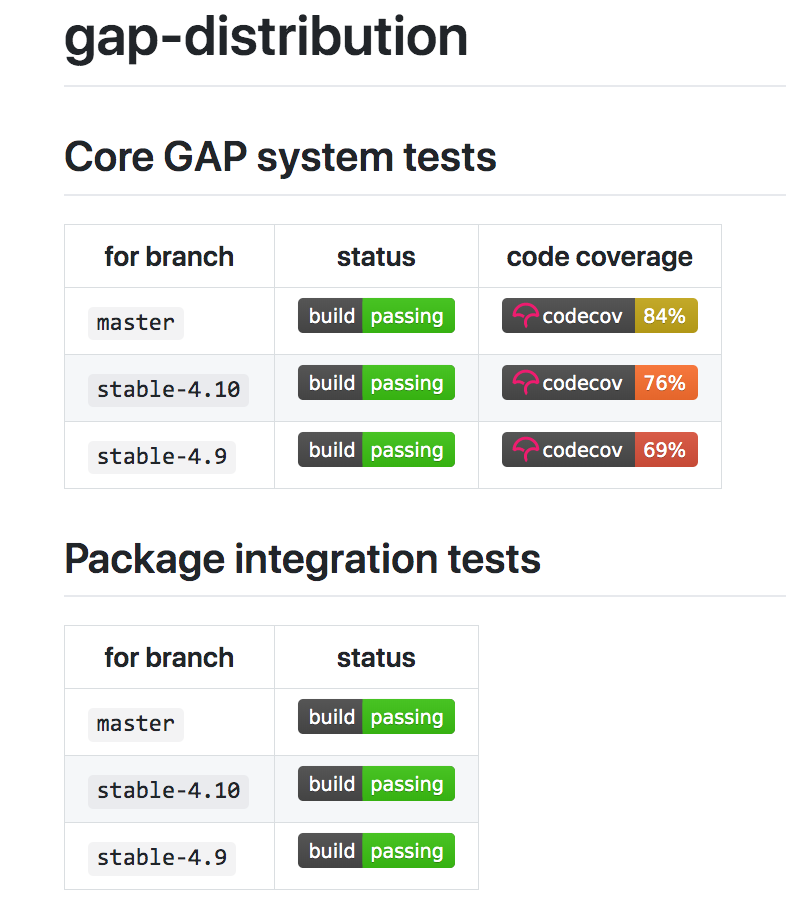
\includegraphics[width=5cm]{images/gap-core-tests}
    \caption{Dashboard with core GAP system and package integration tests}
    \label{fig:gap-core-tests}
\end{figure}

The top part of Figure~\ref{fig:gap-core-tests} shows core system GAP tests,
which are run for every change made to the repository. The bottom part shows
tests which are run once in 24 hours using a Docker container which is built
using a snapshot of the GAP development version on the moment of its creation
and a selection of \GAP packages (including their updates, not yet redistributed
with \GAP). Clicking on the ``status'' button will lead to the overview displayed
on Figure~\ref{fig:gap-docker-master-testsuite}, from where one could inspect
test logs for each of the configurations and see the diagnostics in case of a
test failure.

\begin{figure}[!ht]
    \centering
    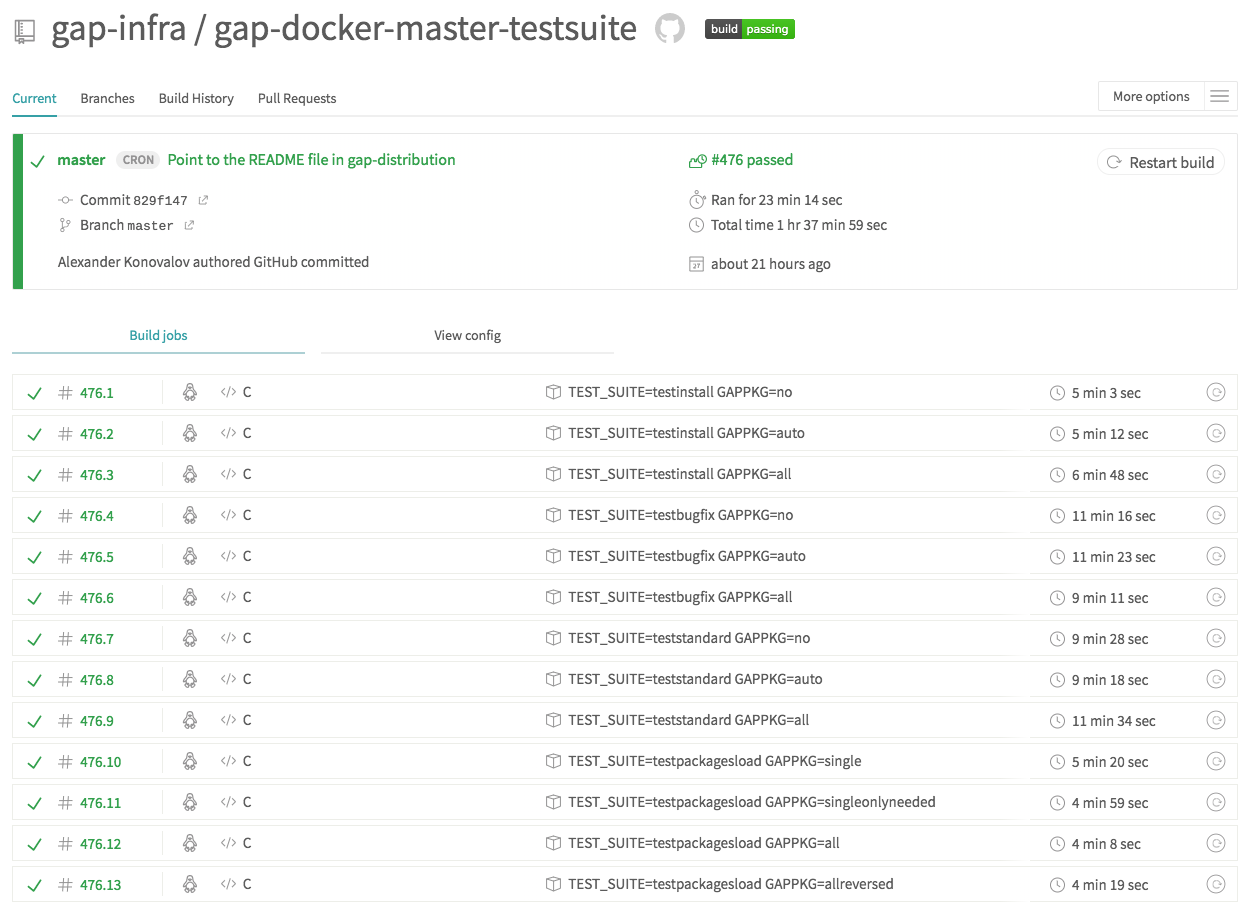
\includegraphics[width=\textwidth]{images/gap-docker-master-testsuite}
    \caption{GAP package integration tests on Travis CI}
    \label{fig:gap-docker-master-testsuite}
\end{figure}

The Docker container for the test displayed on Figure~\ref{fig:gap-docker-master-testsuite}
is one of a set of containers that we maintain for various purposes, from offering 
them as alternative distributions (see Subsection~\ref{distro}) or components for shareable
reproducible experiments (see Section~\ref{demos}), to ways to speed up regression tests running
container-based tests on Travis CI. These containers are publicly available on Docker Hub
(see Figure~\ref{fig:gap-docker}).
\comment{The Docker stuff might deserve to be its own section}

\begin{figure}[!ht]
    \centering
    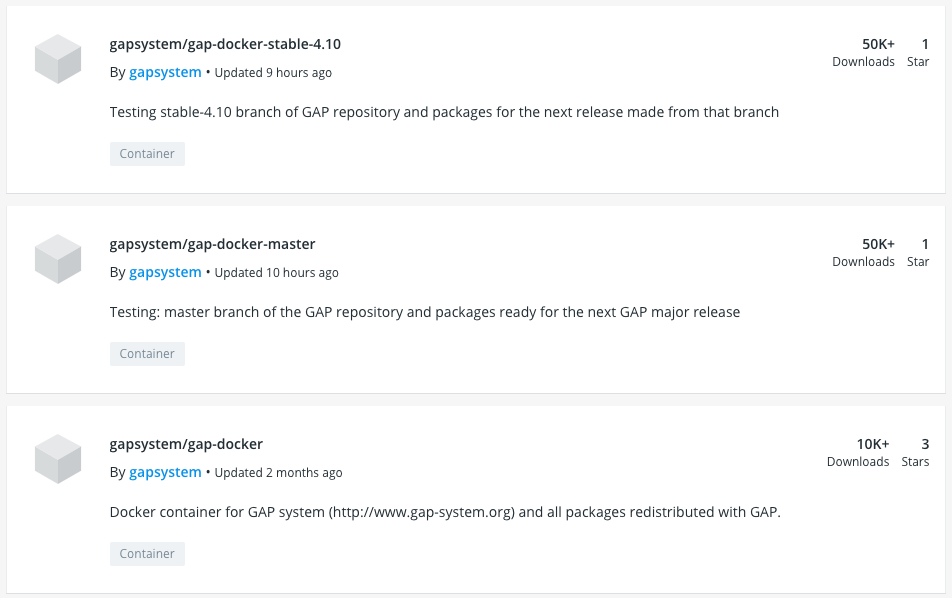
\includegraphics[width=12cm]{images/gap-docker}
    \caption{Selected \GAP Docker containers on Docker Hub}
    \label{fig:gap-docker}
\end{figure}

At the same time, we continue to use Jenkins installation in St Andrews 
for daily and weekly tests, running package updates system, wrapping and
testing release candidates and other tasks. It is also very valuable since 
it does not impose time limits on output inactivity and the overall duration
of the job; second, it allows us to log in into the test workspace for
debugging; third, with the specific \GAP setup for Windows we build it on a
machine with a Cygwin installation, and then install it on a clean Windows
machine to test there. 

\section{\GAP Packages}\label{packages}

Developments, described in the previous section, together with community
supporting activities described in Section~\ref{gap-support}, had substantial
impact on on the health of the package ecosystem. In the duration of the OpenDreamKit
project, we have observed the growth of the number of \GAP packages and package 
authors, improvements in the quality of package testing, more frequent
package updates, and a wide range of tools to help package authors progressed
to a mature state and gained popularity.

First we will introduce these tools, and then we will discuss an impact which
they, together with encouraging package authors to use the open development
model, had on the package authors community.

Our collaborator Max Horn (University of Siegen) developed {\sf ReleaseTools}
(\url{https://github.com/gap-system/ReleaseTools/})
-- a set of scripts to help package authors with the process of making new 
releases. This tool automates all steps of publishing a release for a \GAP package
hosted on GitHub. Without such a tool, making a release involves a lot of steps
and it is quite easy to overlook some of them if one only makes a release from 
time to time; the correction may require even more work. Using {\sf ReleaseTools},
a release may be published in a several minutes with a single call of the release
script, and package authors do not have an obstacle preventing them from publishing
releases more often.

{\sf ReleaseTools} works in conjunction with {\sf GitHubPagesForGAP}
(\url{https://github.com/gap-system/GitHubPagesForGAP}). Using the
latter, one can quickly set up a website for a \GAP package which has
a GitHub repository. This website will be hosted on GitHub pages,
and will be updated each time when the author uses {\sf ReleaseTools}
to publish a new release. All information on the package
website will be automatically updated from the metadata provided by
the package. This greatly simplifies the procedure and helps to keep 
the package website up-to-date.

The \GAP package {\sf Example} by Werner Nickel, Greg Gamble and
Alexander Konovalov \cite{example}
is an example of a \GAP package which may be used as a template for 
a new package. During the reported period, it has been regularly updated
to keep up with the updates of the packages infrastructure. It
switched to using {\tt TestDirectory} to demonstrate how to use 
multiple test files in a GAP package, and migrated
to GitHub, using {\sf ReleaseTools/GitHubPagesForGAP}
for new releases. The guidance for package authors, formerly offered
as an appendix to the {\sf Example} package manual, was moved to the GAP
Reference manual in \GAP~4.9 release. Finally, the {\sf Example} package
demonstrates how to set up Travis CI and CodeCov. Package authors
may copy its configuration files and adapt them with minimal changes.

As an alternative, to create a new package
\GAP users may use another tool called {\sf PackageMaker},
also by Max Horn (\url{https://github.com/gap-system/PackageMaker}). This is
a \GAP package (not redistributed with \GAP, so one should install it
separately), which provides a ``PackageWizard'' - a tool which asks questions
about the intended package, and then creates a new directory populated with 
all the files needed for the start.

\GAP packages should provide documentation. It is possible to use several
formats, one of them is obsolete, originating from the deprecated 
manual format used by GAP in the past, but still in use by 32 packages.
% https://github.com/gap-system/gap-distribution/issues/49
A newer one is an XML-based format which is used for the main \GAP manuals
and requires {\sf GAPDoc package} to build the documentation. Writing XML
code by hand is very tedious and error-prone, and in 2012 Sebastian Gutsche 
and Max Horn (presently both at the University of Siegen) started an 
{\sf AutoDoc} package \cite{autodoc}.
This package allows to create documentation from source code comments
without writing XML files, and then automatically generates XML input
for GAPDoc. By now, this package became very flexible and reliable, and
has been already picked up by 89 GAP packages for building 
some parts or their whole manuals.
% the number 89 was determined by 
%
% grep 'AutoDoc(' */makedoc.g | wc -l
%
% a note "parts or their whole manuals" is essential - 
% it is possible to build a GAPDoc manual using AutoDoc
% and automatically generate title page, updating the
% metadata from those in PackageInfo.g, avoiding the need
% to duplicate details in two places. The rest of the
% manuals for such packages may still remain in XML.

The Docker containers for the latest \GAP public release and for the
development branches of the \GAP repository on GitHub, described in
Section~\ref{gap-infra}, enabled us to make results of regression
tests for \GAP packages easily available to their authors. First,
using a prebuilt docker image does not require to compile GAP and 
packages for each separate test configuration. Therefore, we may
have a separate test configuration for each package. Second, we 
can make test results available to package authors on the Travis CI
website, and ease navigation due to one configuration per package,
so the authors can navigate to the package of their interest.
Finally, we put packages with passing and failing tests into different
Travis jobs, and use that to monitor their status and check that
changes in GAP do not break package tests. 

Figure~\ref{fig:gap-docker-pkg-tests} shows a fragment of the dashboard
from \url{https://github.com/gap-system/gap-distribution} which 
indicates tests status. In this situation, it happened that a fresh
change in the master branch broke tests in one of the packages;
\comment{In fact, in this particular case changes in \GAP were made that 
an empty list no longer qualifies as legal input to {\tt IsDiagonalMat},
but that was used in the {\sf Cryst} package}
the author was immediately notified and reacted with a quick fix.

\begin{figure}[!ht]
    \centering
    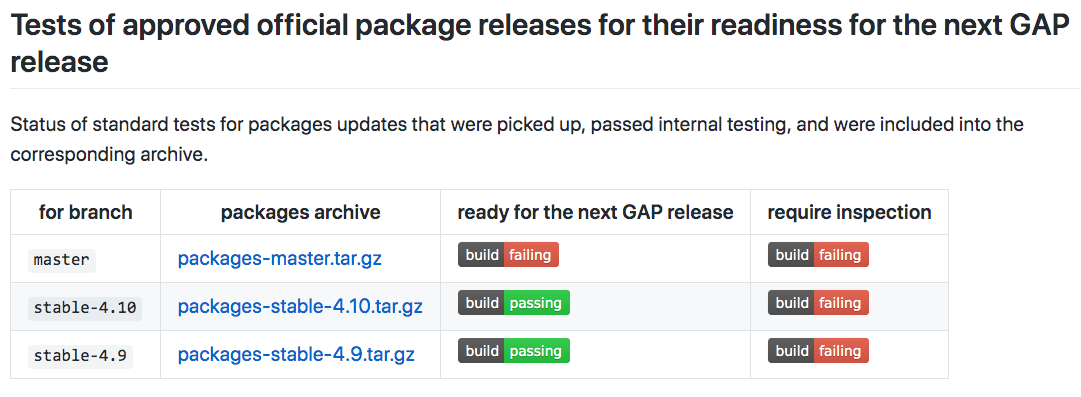
\includegraphics[width=\textwidth]{images/gap-docker-pkg-tests}
    \caption{Dashboard for Travis tests of \GAP packages (GitHub view)}
    \label{fig:gap-docker-pkg-tests}
\end{figure}

The setup for such tests is organised in the gap-infra GitHub organisation
(\url{https://github.com/gap-infra}. Figure~\ref{fig:gap-infra-travis} shows a 
screenshot of a dashboard which indicates tests status.
\comment{All these screenshots may be superfluous - I made them to show
what could be included, we can remove some or cut parts of them out later}

\begin{figure}[!ht]
    \centering
    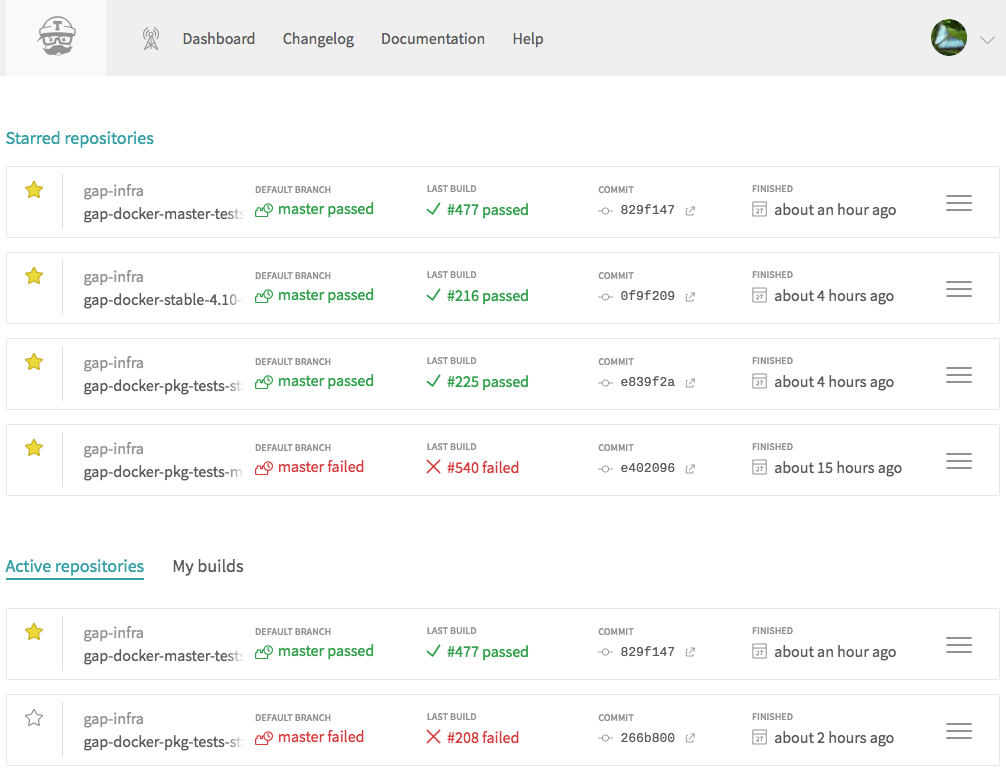
\includegraphics[width=\textwidth]{images/gap-infra-travis}
    \caption{Dashboard for Travis tests of \GAP packages (Travis CI view)}
    \label{fig:gap-infra-travis}
\end{figure}

One of the extensions of the package testing framework, greatly 
facilitated by packages migrating to GitHub, was adding tests not
only for the latest official releases of GAP packages, but also
for their \emph{development} versions.
% https://travis-ci.org/gap-infra/gap-docker-pkg-tests-stable-4.10-devel
% https://travis-ci.org/gap-infra/gap-docker-pkg-tests-master-devel
In this case, the onus to check tests outcomes is on package authors,
and they are able to see how the changes that they have made to
a package but not released yet work in different settings (stable/master,
with default/without/with all packages).

Figure~\ref{fig:gap-packages-travis} shows a screenshot of a 
report on the activity in the gap-packages organisation 
for the last month (for the current version of 
this report, check \url{https://travis-ci.org/gap-packages?tab=insights}).

\begin{figure}[!ht]
    \centering
    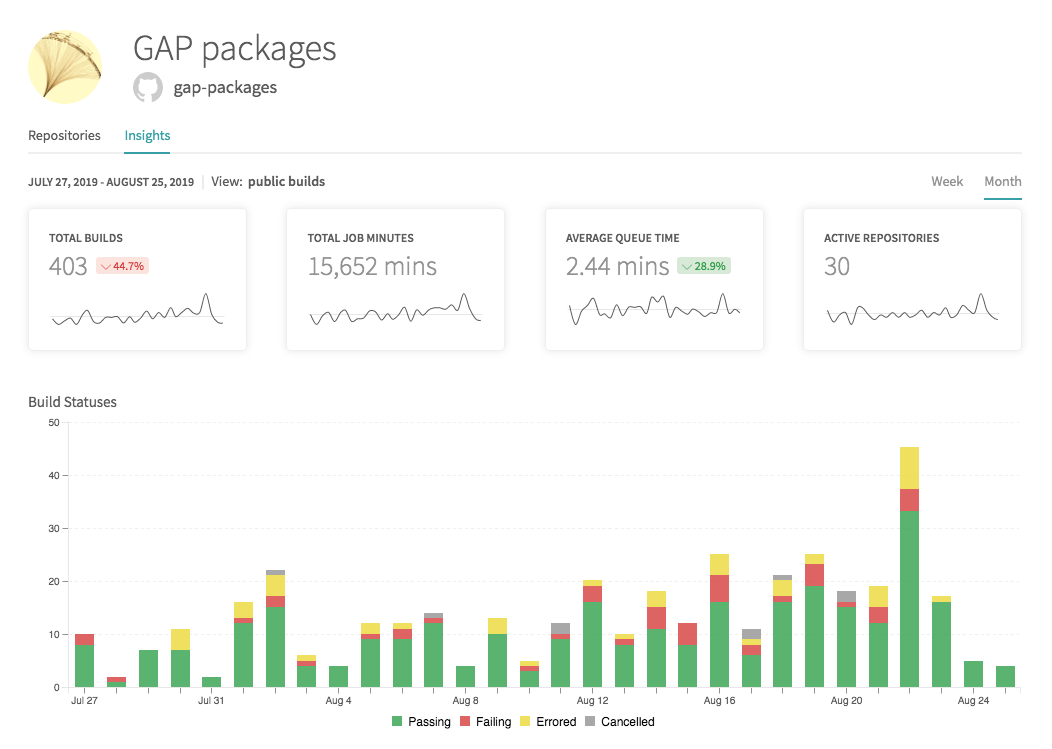
\includegraphics[width=\textwidth]{images/gap-packages-travis}
    \caption{Activity of Travis tests in gap-packages GitHub organisation}
    \label{fig:gap-packages-travis}
\end{figure}

Finally, Figure~\ref{fig:gap-packages-codecov} show the code coverage
leaderboard. We aim at ensuring that code coverage for packages is 
not worse than for the core GAP system, but packages presented there 
put a lot of efforts in ensuring that their coverage is close to 100\%. 

\begin{figure}[!ht]
    \centering
    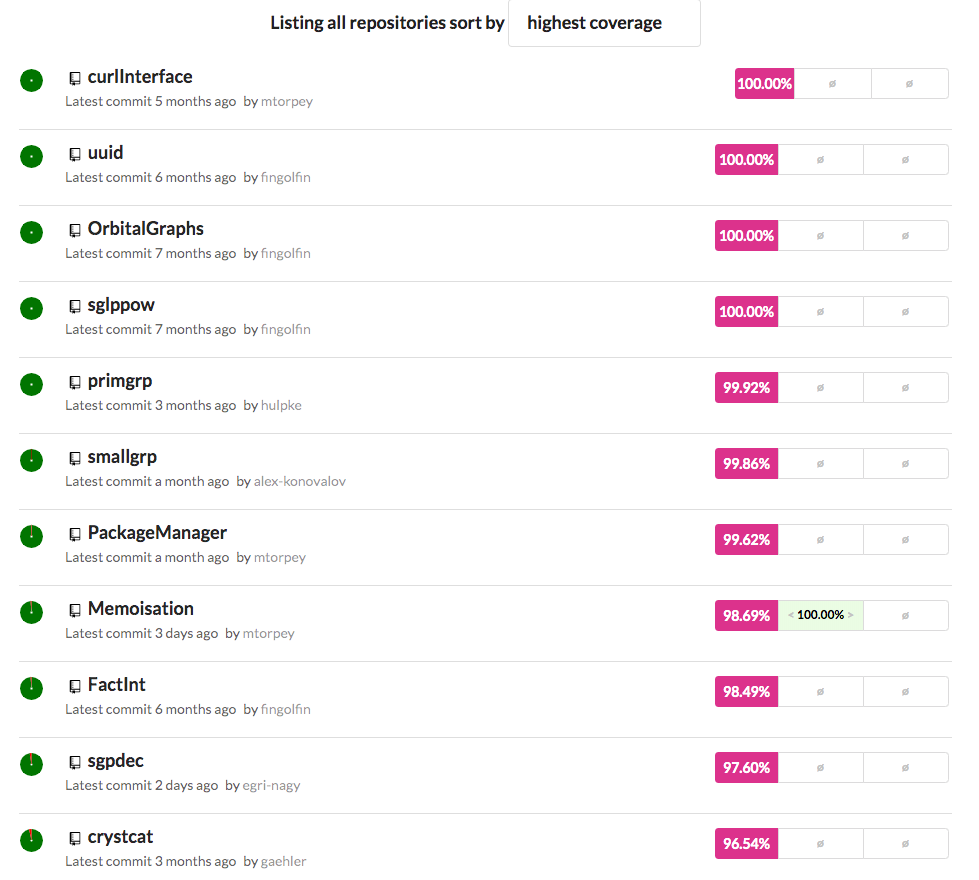
\includegraphics[width=\textwidth]{images/gap-packages-codecov}
    \caption{Codecov leaderboard for in gap-packages GitHub organisation}
    \label{fig:gap-packages-codecov}
\end{figure}

Presently, only 4 packages redistributed with GAP do not have a public 
source code repository. To compare, in October 2018 there were 23 such 
packages. In some cases, that involved non-trivial efforts to establish 
contacts with authors who left academia, getting their permission and 
establishing package license, populating a new repository with releases 
history using archives of past releases, and adopting the packages to
be collectively maintained by the GAP Group. This helps to preserve the
code, reproduce past experiments, eventually find those who may be interested
to take it over.

Figure~\ref{fig:gap-package-releases} shows the number of \GAP packages
included in some \GAP release and their distribution by the year of their
release. At the beginning of the project, GAP 4.7.9 published in November
2015 included 119 packages, 52\% of which were released in 2014--2015.
Now, GAP 4.10.2 included 145 packages, 88\% of which were released in
2018--2019. The ``long tail'' of packages that haven't been updated for
a long time is gradually reducing (we take measures of not breaking
existing functionality, but old packages are usually not picking up
new improvements; and may prevent us from withdrawing obsolete
functionality). Larger proportion of recent releases means that 
packages are updated to make use of the recent \GAP developments,
they are responsive to reports about detected problems; hosting packages on GitHub
facilitates that; we can help by submitting PRs and publish releases for authors,
who prefer to overlook mathematical functionality and general development of the
package but do not want to dive into technicalities of release wrapping.

\begin{figure}[!ht]
    \centering
    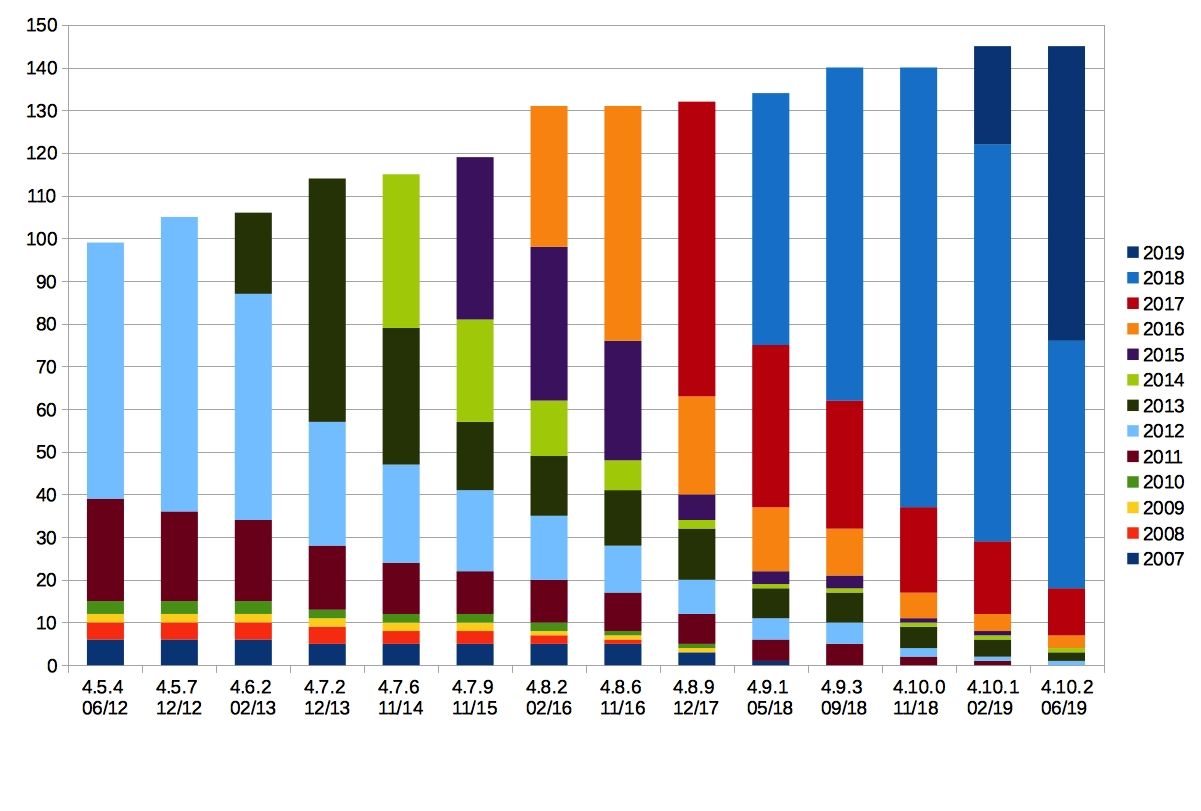
\includegraphics[width=\textwidth]{images/gap-package-releases}
    \caption{Number of \GAP packages and their release year}
    \label{fig:gap-package-releases}
\end{figure}

Moving to GitHub made it easier to start a new package, and to 
get new contributors to existing packages. As Figure~\ref{fig:gap-package-tests}
shows, the number of packages authors increased from 158 in
November 4.7.9 to 196 in June 2019. 

\begin{figure}[!ht]
    \centering
    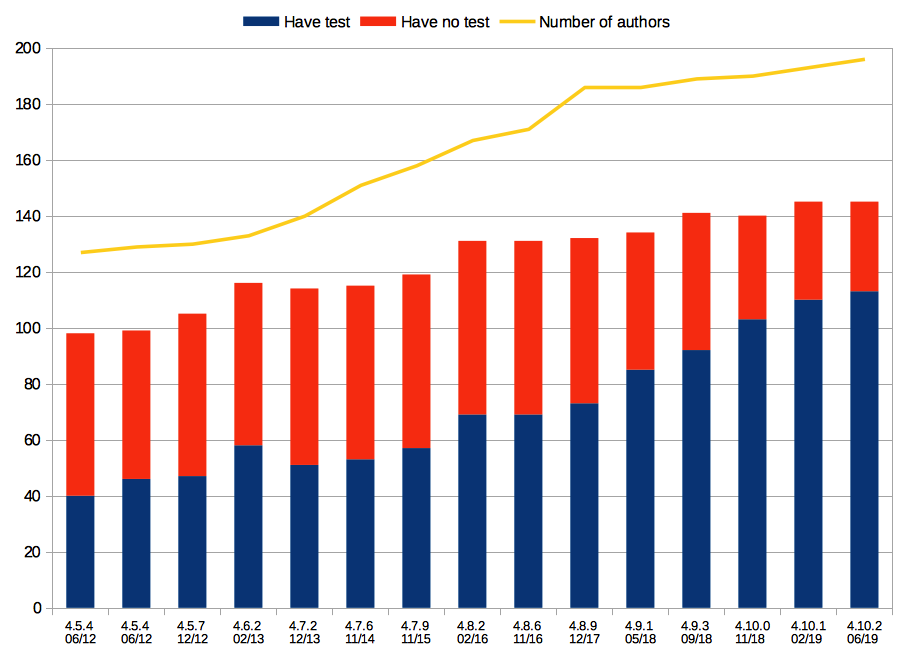
\includegraphics[width=\textwidth]{images/gap-package-tests}
    \caption{Number of \GAP packages, their authors, and packages with tests.}
    \label{fig:gap-package-tests}
\end{figure}

Over the same time, not only package releases became more frequent, but also their quality
improved. If in November 52\% of packages did not provide a standard 
test at all, presently 78\% of packages do have a standard test 
% https://github.com/gap-packages/gap-packages.github.io/issues/9
so their authors are responsible for regular testing them 
with GAP releases and development versions.
Some of them use their own setup for continuous integration
(like e.g. the \href{https://homalg-project.github.io/}{\sf homalg} project,
which uses \href{https://circleci.com/}{CircleCI}).

At the moment of writing, in the stable-4.10 branch,
standard tests pass for 102 packages
% https://travis-ci.org/gap-infra/gap-docker-pkg-tests-stable-4.10
and fail for 12.
% https://travis-ci.org/gap-infra/gap-docker-pkg-tests-stable-4.10-staging 
(it may be worth to note what "fail" means - not serious bugs
but different output, or incompatibility with some other package
not loaded by default).

\subsection{\GAP package manager}\label{pkg-manager}

WHO: Michael

For many years, the installation of packages in \GAP has been an entirely manual
process.  If a user requires a package that is not currently installed on their
system, they are required to visit the \GAP website, or the website of the
required package, download an archive or repository and extract it into their
package directory.  In many cases, they must also compile the package before
use, in a process that is not consistent between packages.  Worst of all, any
dependencies must also be installed individually, including all these steps for
each one.

This awkward installation procedure is mitigated by the inclusion of a large
number of packages with the main release archive (145 packages were included
with \GAP 4.10.2).  This solution masks the problem for the majority of users,
who do not require any more specialised packages.  However, it also results in a
1.6 GB standard installation, of which the packages make up 1.4 GB.  Many of
these packages will never be loaded by a given user. \TODO{Adding
  packages as a user to a central installation. Installing development
  versions of packages}

The possibility of a more sophisticated package management system for \GAP has
been discussed for some time, and was realised with the creation of {\sf
  PackageManager} (\url{https://gap-packages.github.io/PackageManager/}) in
September 2018, by Michael Torpey.  Development started after a discussion at
\GAP Days Fall 2018 (\url{https://www.gapdays.de/gapdays2018-fall/}) and an
initial release was made before the end of that meeting.  New features have been
added in various further releases across the past year.

{\sf PackageManager} is a \GAP package itself, which is operated from inside a
\GAP session.  This approach to package management was chosen over an external
manager, since it allows users to install and remove packages without ever
leaving the environment of the \GAP prompt.  The first advantage of this is that
users have a comfortable environment, without needing to learn how to use
external tools; and the second is that, in most cases, packages can be installed
and loaded without restarting the session as in Figure \ref{fig:pkgman-sample},
meaning that users' workflow is interrupted as little as possible, and they do
not need to save and reload their work.

\begin{figure}[!ht]
    \centering
    {\tiny
\begin{verbatim}
gap> InstallPackage("digraphs");
#I  Getting PackageInfo URLs...
#I  Retrieving PackageInfo.g from https://gap-packages.github.io/Digraphs/PackageInfo.g ...
#I  Downloading archive from URL https://github.com/gap-packages/Digraphs/releases/download\
/v0.15.4/digraphs-0.15.4.tar.gz ...
#I  Saved archive to /tmp/tmcLM2FI/digraphs-0.15.4.tar.gz
#I  Extracting to /home/user/.gap/pkg/digraphs-0.15.4 ...
#I  Checking dependencies for Digraphs...
#I    io >=4.5.1: true
#I    orb >=4.8.2: true
#I  Running compilation script on /home/user/.gap/pkg/digraphs-0.15.4 ...
true
gap> LoadPackage("digraphs", false);
true
\end{verbatim}
    }
    \caption{Installing a package using {\sf PackageManager}.}
    \label{fig:pkgman-sample}
\end{figure}

The main functions provided by {\sf PackageManager} are \texttt{InstallPackage},
\texttt{UpdatePackage}, and \texttt{RemovePackage}.  The first,
\texttt{InstallPackage}, takes a string which can be any of several different
forms: the URL of an archive, repository, or package info file, or simply the
name of a package.  In the case of a URL, the appropriate file is retrieved
using an internet connection, and used to install the package; if a package name
is given, it is looked up in a pre-defined list of package URLs and installed
from there.  In most cases, the latest released version of a package is
installed; a user can specify an older version by giving an explicit archive
URL, or a development version by specifying a branch along with the url of a
version control repository.  % currentPackageInfoURLList

The ability to install a package given only its name is useful, but requires
some important design decisions: how do we decide which packages to support, and
which versions do we install by default?  One option would be to have a
centralised repository (as is common for the {\sf APT} package manager) which
contains a carefully checked set of package versions that are known to work with
the installed version of \GAP and with each other; this has the advantage of
stability and control, but may make it harder to get the latest software
versions.  The other option is to store links to appropriate locations on the
package websites, allowing the most recently released version to be installed
without explicit approval from the \GAP authors; this approach is closer to the
more liberal {\sf pip} package manager for the Python language.
In the end, the latter approach was taken for the following reaons:
\begin{itemize}
\item approved package versions for a given release are likely to be included
  with the \GAP installation anyway, and so it is unlikely that users would need
  to reinstall these;
\item it requires no additional infrastructure, since a
  \texttt{currentPackageInfoURLList} is already maintained for testing purposes;
\item it encourages active use, and therefore testing, of recent releases.
\end{itemize}
This decentralised approach has therefore been adopted for the moment, though
future development could move easily towards a different approach.

Over the course of {\sf PackageManager}'s development, it has accumulated
various features that automate as much of package installation as possible:
\begin{itemize}
\item any kernel module is configured and compiled, if present;
\item package documentation is built from source if necessary;
\item prerequisites are installed using \texttt{prerequisites.sh} if present;
\item all missing package dependencies are installed, or recompiled if broken;
\item basic checks are performed to verify that installation was successful.
\end{itemize}
This has resulted in a reasonably smooth installation process, with very little
friction encountered by a user who tries to get a new package working.  It is
now a deposited package in \GAP, and is therefore distributed in the main
archive with each release.

\TODO{Mention that it uses ~/.gap ?  Or is that too technical?}

\begin{itemize}
  \item The package manager is now on CoCalc (as part of GAP 4.10.2) which enables each user to install the packages they
    need, rather than forcing CoCalc operators to manage these
    installations separately. Example of positive two way interaction
    with CoCalc.
\end{itemize}

\subsection{Packaging \GAP distribution}\label{distro}

WHO: Alex

\comment{See the Release checklist at \url{https://github.com/gap-system/gap-distribution/blob/master/DistributionUpdate/RELEASE_CHECKLIST.md}
Some text below pasted from there, needs shortening}

We aim at making a minor release every several months and a major 
release once or twice per year. 

Actual schedule may be corrected - critical bug fixes may need 
an urgent minor release, and substantial changes may require 
more time for a major release.

Usually, if a previous minor release has been made a couple of 
months ago, and there is a substantial amount (say, 15 or more) 
of updated packages and/or changes in the core \GAP system, 
there may be a time for a release.

Figure~\ref{fig:gap-package-releases} shows the number of minor
and major \GAP releases per year, starting from the release of
\GAP~4.4 in 2004.

\begin{figure}[!ht]
    \centering
    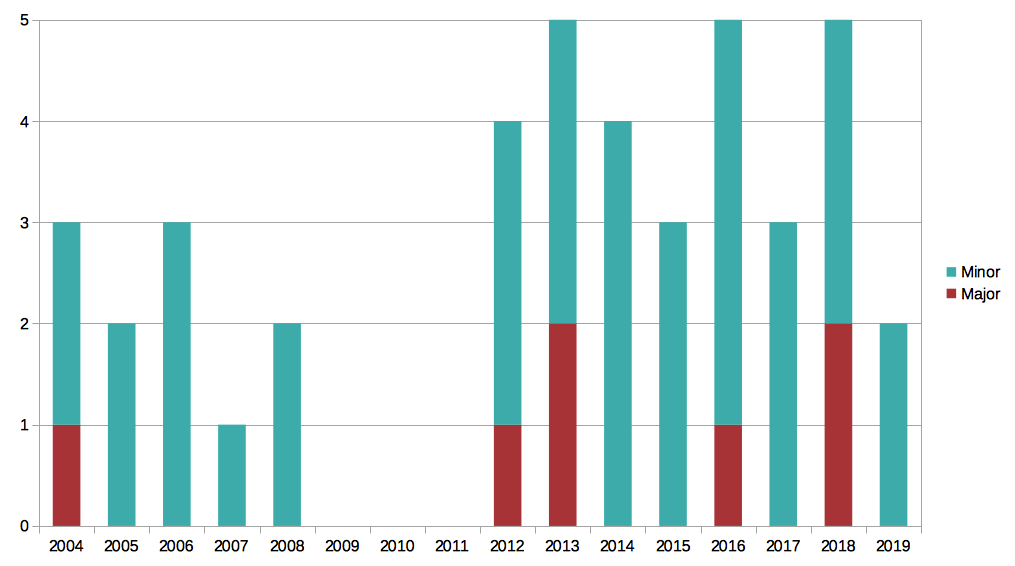
\includegraphics[width=\textwidth]{images/gap-releases}
    \caption{Number of major and minor \GAP releases per year since \GAP 4.4 release.}
    \label{fig:gap-releases}
\end{figure}

\TODO{Say something about this: as noted in GAP 4.10 description, 
better testing tools and increased thoroughness of package testing 
allowed us to concentrate on the changes in the master branch
(which is a prototype for the next major release), and limit 
the changes in the current release branch to bugfixes and selected 
non-disruptive changes backported from the master branch.
(Indeed, less situations when package authors reported to us after 
the release that we broke their package - this can be now detected 
earlier). One could try to look at the descriptions and number of 
changes in the release overview to see that. Also, if formerly we provided
a beta release and were giving to package authors a 2-months window to
test and update their packages, then the need in doing this disappeared
with the improvements of the testing, and for the first time in GAP 4.10.0
we did not provide a beta release but published GAP 4.10.0 straightforwardly.
This went well - GAP 4.10.1 was published in due course in February 2019,
without any rush.}

Release wrapping and automated testing is performed in St Andrews
using the Jenkins automation system. \GAP distribution is tested
in various combinations of operating systems (Linux, macOS, Windows)
and build modes (32-bit and 64-bit), and with different sets of
loaded packages. Automated regular testing of the codebase ensures
that we can release as often as deemed necessary. Modern version
control system helps us to have release branches and a master branch
where we accumulate things for the next major release, and then
create the next release branch for things to stabilise and let package
authors to test it and if need be adapt their packages.

\GAP distribution is provided in several archive formats for Linux and macOS,
and in zip archives and as an executable installer for Windows.
We also provide several auxiliary archives which keep the core system
and packages separately - these are used by providers of alternative
distributions, systems which use \GAP (such as SageMath and OSCAR)
and for testing.

\GAP alternative distributions include the Docker container for the 
latest public \GAP release (\url{https://hub.docker.com/r/gapsystem/gap-docker/},
and a so called ``tap'' for the Homebrew package manager for macOS
(\url{https://github.com/gap-system/homebrew-gap}). 

It is also possible to try \GAP online in a Jupyter notebook running 
on Binder, following instructions from the README file in the repository
located at \url{https://github.com/gap-system/try-gap-in-jupyter}.

One could also use \GAP via a free or paid account
on \href{https://cocalc.com/}{CoCalc} (formerly SageMathCloud).
The user should be aware that the combination of \GAP packages 
available there may differ from the one from the official \GAP distribution.

\section{Jupyter interface to \GAP}\label{sec:jupyter}

WHO: Alex, with help from and Michael
Need to explain why this is not in WP3 deliverables?

TODO: Refer to previous deliverables and describe how their outputs
evolved and any impacts they achieved

JupyterKernel has been reported in DX.Y. Since that, there were
several more releases of the kernel, associated with new \GAP
releases, improving its robustness. 

JupyterKernel lead to several follow-up developments, their
functionality will be described below: Francy, JupyterViz,
other work by Nathan Carter (also mention related work on
GroupExplorer).

Have used in in teaching and in explaining how to share 
reproducible experiments that use \GAP. Using Binder
allows to try \GAP in Jupyter online. Provide details
and consider including an appendix with an example 
demonstrating the setup.

\section{Community building, Technical support, User Training and Dissemination}\label{gap-support}


WHO: Alex

Describe all training events, Software Carpentry lesson, other workshops

Why is this not in WP2 deliverables?

\section{Interfaces, WP6}

WHO: Michael

Fix title of the section.

High-level interoperability

Persistent memoisation

Why is this here and not in a WP6 deliverable?

\section{A collection of demonstrators}\label{demos}

For example:

Reproducible experiments with Jupyter

``full-stack semigroups''

persistent memoisation

databases

\newpage
\appendix

\section{Sharing reproducible computational experiments}

This appendix presents an example of organising GAP code 
and data to give others an opportunity to inspect them and rerun
the computation on a freely available called \href{https://mybinder.org/}{Binder}.

It demonstrates integration of a number of concepts mentioned
in the report: GAP regression testing; setup for continuous
integration and code coverage reports; Docker containers with
the GAP distribution; and GAP Jupyter interface.

For this demonstrator, we collaborated with the authors of \cite{black-box} 
who worked on the code for this paper in the GitHub repository located 
at \url{https://github.com/sukru-yalcinkaya/unipoly} in the file 
called {\tt unipoly.g}.

This code does not justify the creation of a new GAP package, 
but it can reuse packages setup for Travis CI and Codecov by 
creating a {\tt tst} directory with the test files and adapting
{\tt .travis.yml} and {\tt .codecov.yml} configuration files
from the \GAP package {\sf Example}. Importantly, it also
allows to check that the code works in GAP 4.9, GAP 4.10 and 
the master branch of the GAP repository, which is a prototype for
GAP 4.11.

\begin{figure}[!ht]
    \centering
    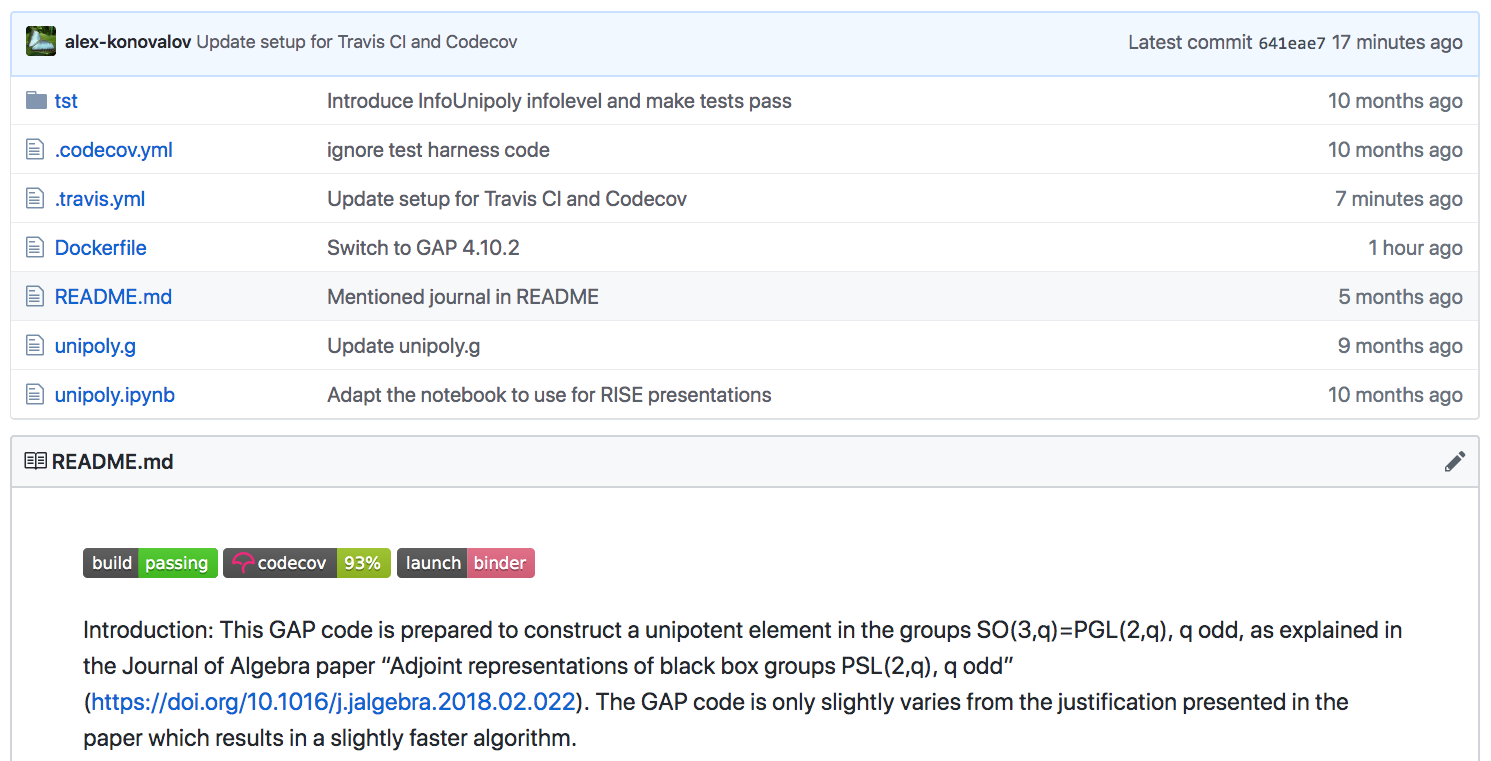
\includegraphics[width=\textwidth]{images/unipoly-repo}
    \caption{unipoly project repository}
    \label{fig:unipoly-repo}
\end{figure}

The next step is to produce a Jupyter notebook which combines input,
output, and textual narrative in one document. The notebook contains
the {\tt Read(unipoly.g);} command to read the code first. This is
a good practice for organising reproducible experiments: keeping the
code in a single location in a {\tt .g} file allows its reuse and
automated testing, and avoids code duplication. 

When the authors prepared and committed the Jupyter notebook describing
their calculation, they are ready to share it on
\href{https://mybinder.org/}{Binder}. First they need to add 
to their repository a {\tt Dockefile} with the following content:

{\tiny
\begin{verbatim}
FROM gapsystem/gap-docker

MAINTAINER Alexander Konovalov <alexander.konovalov@st-andrews.ac.uk>

COPY --chown=1000:1000 . $HOME/unipoly

RUN sudo pip3 install ipywidgets RISE

RUN jupyter-nbextension install rise --user --py

RUN jupyter-nbextension enable rise --user --py

USER gap

WORKDIR $HOME/unipoly
\end{verbatim}
}

This file builds a Docker container based on the container {\tt gapsystem/gap-docker}
with the latest GAP release, which we provide as an alternative GAP distribution
(see Subsection~\ref{distro}). Additional commands specify how to copy the code into
the new container, and install additional extensions for Jupyter-based slideshows.

After that one should follow \href{https://mybinder.org/}{Binder} instructions to
set up a new Binder project. A completed setup will allow to click on the ``launch binder''
button in the README file on GitHub (as seen on Figure~\ref{fig:unipoly-repo}
to start a Jupyter notebook server in the cloud,
either using a prebuilt image of the project or by building a new one in case of any
changes in the GitHub repository. When the server will be started, it will display
a file browser as shown on Figure~\ref{fig:unipoly-files}.

\begin{figure}[!ht]
    \centering
    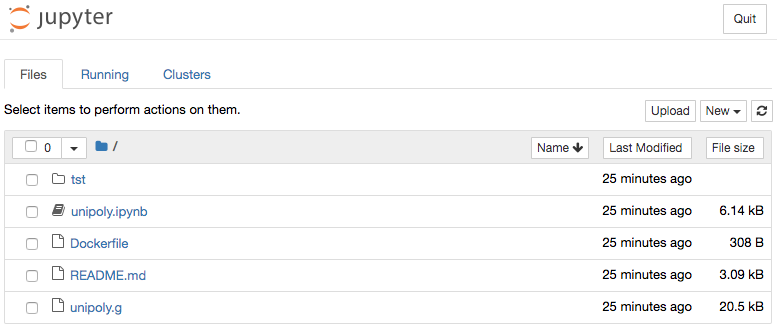
\includegraphics[width=\textwidth]{images/unipoly-files}
    \caption{File browser running on Binder}
    \label{fig:unipoly-files}
\end{figure}

Clicking on {\tt unipoly.ipynb}, the user will open the Jupyter notebook
and will be able to rerun it as shown on Figure~\ref{fig:unipoly-notebook}.

\begin{figure}[!ht]
    \centering
    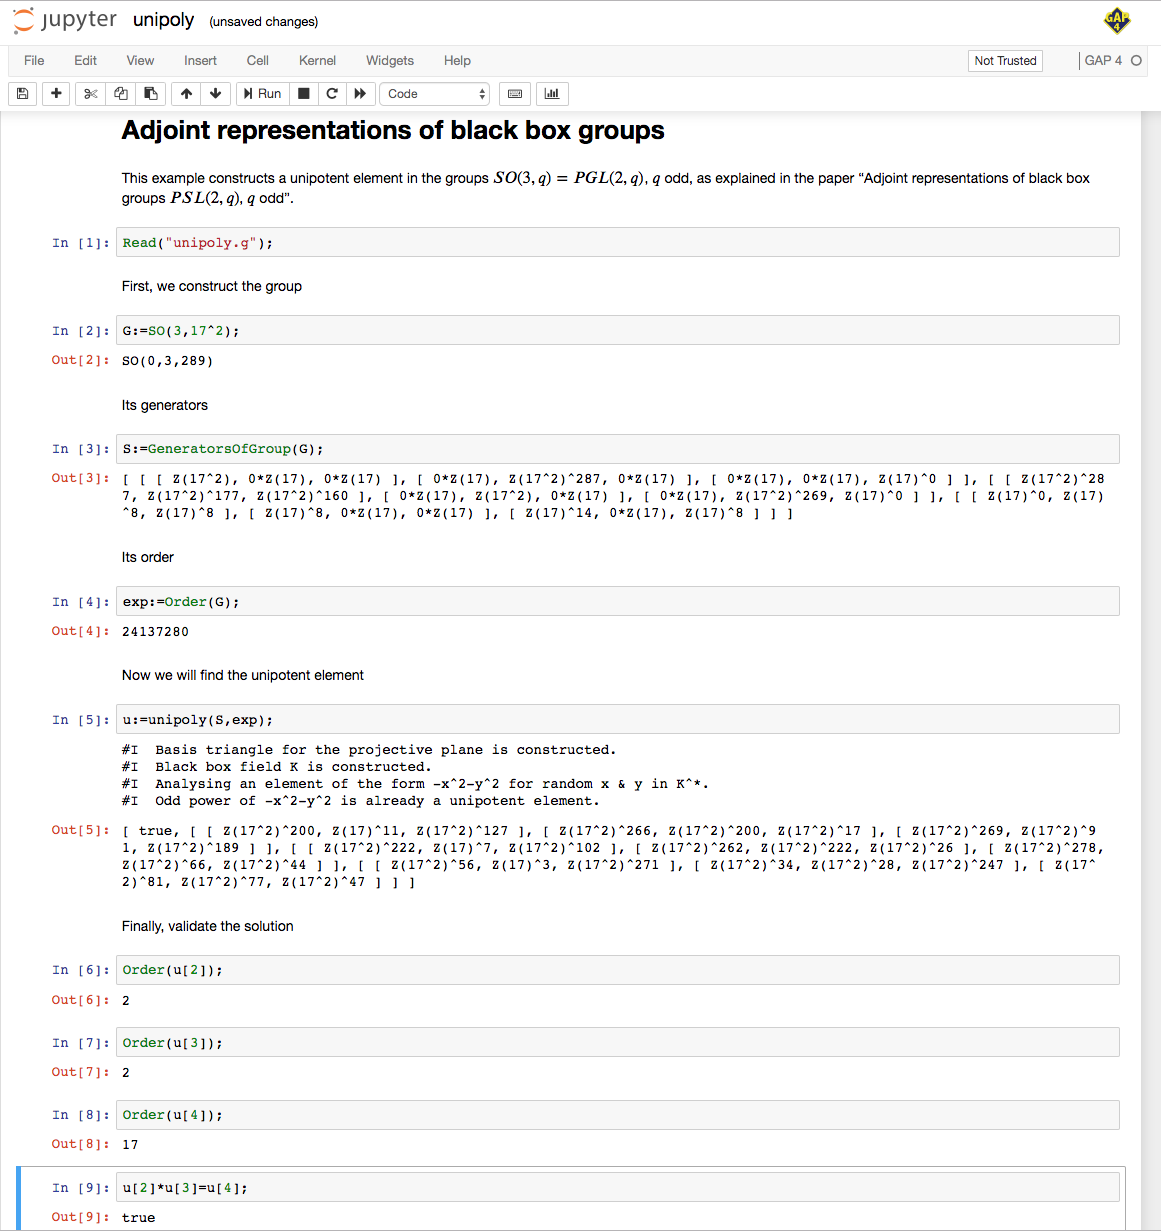
\includegraphics[width=\textwidth]{images/unipoly-notebook}
    \caption{Jupyter notebook running on Binder}
    \label{fig:unipoly-notebook}
\end{figure}

One could also switch to the slideshow mode (the notebook would require
some configuration to explain which cells should be displayed on the
same slide and which not), and run an interactive presentation, as
as shown on Figure~\ref{fig:unipoly-slide}.

\begin{figure}[!ht]
    \centering
    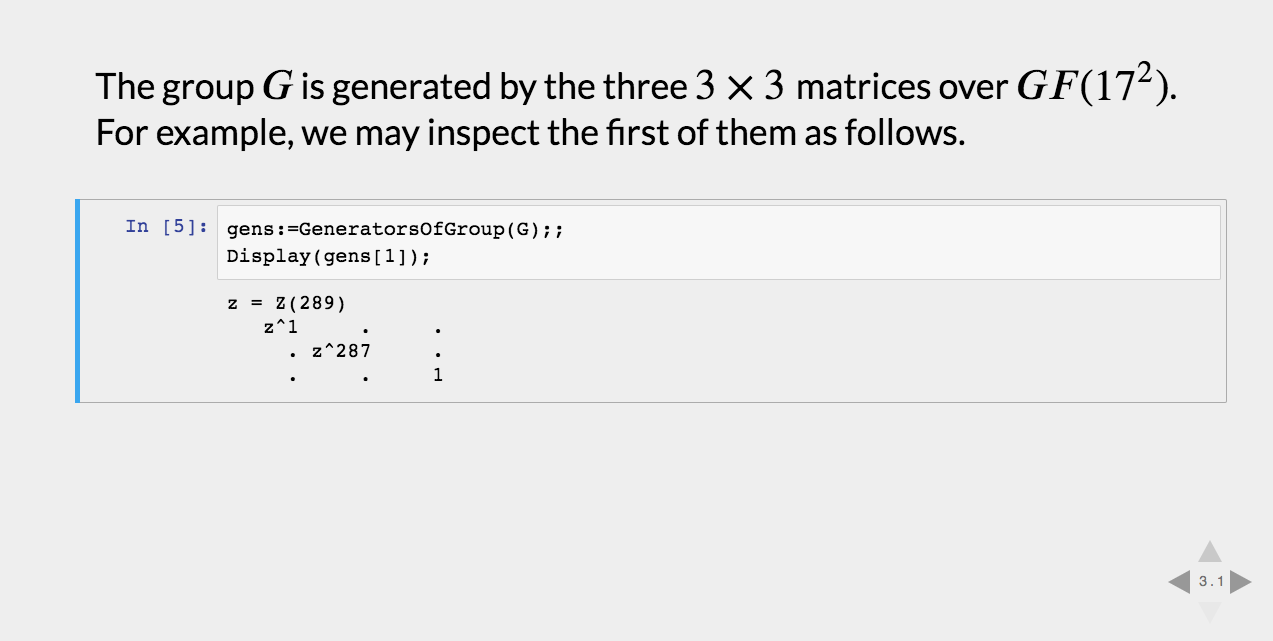
\includegraphics[width=\textwidth]{images/unipoly-slide}
    \caption{Slideshow with interactive computation running on Binder}
    \label{fig:unipoly-slide}
\end{figure}

Thus, connecting the project repository to Binder allows other users
(e.g. readers or referees of the paper) to rerun computations on Binder
without spending efforts on installing all necessary components
(may be hard for them as non experts, may not always be possible;
something may not work on Windows, etc.

\TODO{what are the limitations of Binder and suggested workarounds}

\newpage
\TODO{Ensure that we are following software citation recommendations properly!}
\printbibliography

\end{document}


%%% Local Variables:
%%% mode: latex
%%% TeX-master: t
%%% End:

